%%%%%%%%%%%%%
%
%
% Text for dissertation appendix B and the signal chain response white paper.  
% They will have identical text.
%
% Ben Rotter - University of Hawaii at Manoa - March 2017
%
%%%%%%%%%%%%%%

%	\begin{abstract}
	The generation of a system impulse response for the ANITA3 instrument from pre-flight calibration measurements is required to accurately relate the digitized time series of analog voltages propagated to the detector electronics to the correlating electric field physically transiting the instrument.  As the system is sensitive to a wide bandwidth, a full frequency dependent array of complex phasors is required to completely characterize the system.  The ANITA3 (and more recent ANITA4) flights employ slightly different antennas than the previous ANITA1 and ANITA2 flights.  The purpose of the change was to capture additional sub 200MHz frequency electromagnetic signals.  Additionally, the amplification and filtering chains of the newer flights have undergone subtle modifications that preclude direct relation to those of earlier flights.  This change necessitates a thorough analysis and characterization of the full ANITA3 signal chain, from antenna to digitizer.
%	\end{abstract}
	
\section{Introduction}

	There are two distinct systems on the ANITA3 instrument that alter the received time domain electromagnetic signal prior to digitization: the Seavey horn antennas, and the filtering and amplification network.  The antennas used on the ANITA flight are broad band, with a design bandwidth of 180MHz to 1200MHz, and whose dual orthogonal polarizations have co-located phase centers.  These antennas couple the propagating electromagnetic (EM) radiation emitted by an extensive comic ray or neutrino air shower (EAS) into a 50$\Omega$ transmission line by uniformly transforming the impedance from that of free space to that of the RF system.  The collection of amplifiers, filters, and other 50-ohm RF components that populate the path between the antenna and the LABRADOR chip is colloquially known as the signal chain, and adds additional frequency dependent gain and phase modulation before the signal is finally read out by a fast sampling broad band ADC.  To calibrate these two systems, input signals were injected into the systems and measurements were taken of both the input and output signal on a calibrated oscilloscope.  The methods and techniques used to generate an impulse response using these input and output signals will be discussed, as well as the results for the ANITA3 flight.

\subsection{Discrete Fourier Transform}

	To determine the spectral content of a time domain signal, I have employed the use of a Discrete Fourier Transform (DFT).  Equation \ref{eqn:DFT} \cite{DFT} exhibits a transformation between a discretely sampled time domain signal $x_{n}(t)$ and the equivalent Fourier series $\mathcal{F}_{k}(f)$.  Additionally, Equation \ref{eqn:IDFT} \cite{DFT} shows the inverse of the DFT, with a $\frac{1}{N}$ normalization to preserve reciprocity of the transformations.

\begin{equation}
\mathcal{F}_{k} = \sum_{n=0}^{N-1} x_{n}e^{-2\pi ikn/N}
\label{eqn:DFT}
\end{equation}

\begin{equation}
x_{n} = \frac{1}{N}\sum_{k=0}^{N-1} \mathcal{F}_{k}e^{-2\pi ikn/N}
\label{eqn:IDFT}
\end{equation}


As our measured signal is required to be purely real, the Fourier equivalent series will be hermitian, setting the limits for the sum to purely positive integers.  Additionally, though a true Fourier transform takes the time or frequency integral over its respective range and thus introduces a time multiplication to the resulting unit, the DFT does not have a time normalization, leaving the units of both arrays as Volts.

The effect of transforming from a time series to a Fourier series and back should be zero, however any signal manipulations such as zero padding, up-sampling, or truncating, will have an effect on the opposing Fourier equivalent pair as well.  This can be used to more easily manipulate signals in a manner that matches the physical boundaries of the system.


\subsection{Units and Spectrum Discussion}

	Accurately representing the amount of power in a time domain waveform or network as a function of frequency requires both a normalized Fourier transform as well as the appropriate units.  There are two main types of signals which we are considering in this analysis, absolute measurements, referenced to a measured voltage on constant impedance network, and relative measurements, relating two different measured signals.  
	
	An example of an absolute measurement is the time series waveforms captured on oscilloscopes.  These can be described by decibles referenced to 1mW (dBm), seen in Equation \ref{eqn:dBm}, or Power Spectral Density (PSD), represented by dBm/Hz and seen in Equation \ref{eqn:PSD}.  For the purposes of this analysis, the Power Spectral Density will be used.
	
\begin{equation}
Power(f) = 10log_{10}(\frac{|\mathcal{F}(f)|^{2} * 1000[\frac{mW}{W}]} {Z})\qquad [dBm]
\label{eqn:dBm}
\end{equation}

	
\begin{equation}
PSD(f) = 10log_{10}(\frac{|\mathcal{F}(f)|^{2} * 1000[\frac{mW}{W}]} {Z*df})\qquad [dBm/Hz]
\label{eqn:PSD}
\end{equation}



	The ratio of spectral power between two different signals $x_{A}(t)$ and $x_{B}(t)$, can be done through division of their equivalent Fourier representations $\mathcal{F}_{A}(f)$ and $\mathcal{F}_{B}(f)$.  The logarithmic magnitude of this ratio is what is most often recognized as the gain of the network.  The calculation of the gain is seen in Equation \ref{eqn:gain}.
	
\begin{equation}
Gain(f) = 10log_{10}(|\frac{\mathcal{F}_{A}(f)}{\mathcal{F}_{B}(f)}|^{2}) \qquad [dB]
\label{eqn:gain}
\end{equation}


	An example of relative measurements are network analyzer S21 measurements and transfer functions, which do not quantify an absolute power, only a ratio of powers.  Note that the subtraction of two absolute measurements, regardless of normalization, yields a gain.  Also note the distinction between Equation \ref{eqn:gain}, which measures the logarithmic increase in power, to other quantities commonly referred to as gain which measure the ratio between amplitudes.  In this case, there is a factor of two difference between them.


\section{Seavey Antenna Impulse Response}

	\subsection{Measurement Goals}

	Many calibration measurements were taken for the antennas used in the ANITA3 flight.  Each measurement probed a different characteristic of the antennas, and had various drawbacks and benefits.  There are several major parameters of interest for the antenna measurements. First, the absolute phase and gain response for any incident EM field at the peak response angle.  This angle of peak response, nominally pointed orthogonally to the antenna face, is known as the "boresight" angle, and the resulting quantity is known as the antenna gain, represented in units of dBi and discussed later. The directionality and gain pattern as a function of angle off the maximal transmission and receive direction is directly related to the antenna gain, and is needed to determine amplitudes for signals incident at angles off of the boresight.   Lastly, a measurement of the cross polarization fraction is required to determine the full Stokes parameters of any incident field.  This last measurement has currently not been studied for the ANITA3/4 antennas.
	
	\subsection{Measurements Summary}
	
	Three different measurements of the antennas were taken that are discussed in this paper, each of which probe a unique region of the full calibration measurement.  
	
		\subsubsection{UH Anechoic Chamber}
		First, a measurement was taken at the University of Hawaii at Manoa in a copper lined, RF sealed, anechoic chamber using two "identical" (same model and manufacturing batch) ANITA3 flight antennas.  This measurement allowed a maximally noise free environment in which to measure any small signal effects that may be present in the antennas.  It also removes the requirement for correlation and averaging of multiple waveforms, decreasing uncertainty introduced by interpolation techniques.  Unfortunately, the size of the anechoic chamber forced the distance between the antennas into the near field region for the lower side of the frequency bandwidth.  This causes results below 200MHz, with a wavelength of ~1.6m and minimum far field distance requirement of 3.2m, to be slightly distorted and require near-field Fresnel corrections. As this is the region in which the antennas were supposed to perform differently than previous ANITA antenna designs, this experimental setup and required correction is highly problematic.  Additionally, measurements of the gain pattern far off the maximal bore-sight angle have Fresnel zones occluded by the absorbing material that lined the walls of the chamber, once again introducing Fresnel interference and increasing the uncertainty in the measurements.
		
	
		\subsubsection{UH Rooftop Measurements}
	Additional tests were undertaken at the University of Hawaii with much larger separation distances.  To accomplish this, the two antennas under test were placed on building rooftops separated by a moderately sized courtyard.  The building separation was large enough to escape the near-field of the lower frequency antenna response, yet close enough to preclude any ground bounce interference or multi-path issues.  These measurements were plagued by anthropogenic noise, however a large sample of waveforms uncorrelated to this noise was taken reducing the resulting background significantly.  These measurements provide the best results for the absolute system gain and antenna directivity.
	
		\subsubsection{Palestine TX 2014 Antenna Consistency Checks}
	Finally, for the full ANITA flight the consistency and similarity of all 48 antennas needed to be measured.  Bore-sight gain measurements were taken for all antennas at the Columbia Scientific Balloon Facility (CSBF) in Palestine TX during the 2014 integration campaign of the ANITA3 payload.  This was done in a CSBF balloon hangar, is used in this analysis, and is detailed in the following section.
	
	Due to the physical and engineering limitations of the experimental apparatus, one of the antennas had to be flipped in relation to the other, causing the approximation of identical antennas to lose some justification.  This introduces several issues.  First, there will be a polarity flip of the measured signal.  This can be easily handled by multiplying the measured time series by -1, re-inverting the signal.  A worse problem occurs when the peak power angle of the antenna beam "wanders" away from the boresight.  In the case where the antennas were oriented symmetrically to each other, an antenna height that peaked at a location other than the boresight angle would not distort the measurement.  However, when the antennas are oriented in a flipped configuration, any angular deviation of the peak antenna pattern will be squared as each antenna contributes its own angular deviation.  
	
	
	
	\subsection{Absolute Boresight Complex Antenna Height}
		
		The relationship between the magnitude of an electric field vector and the induced potential on the transmission line output of the antenna is a combination of the radiation efficiency and beam pattern, and is colloquially known as the complex antenna height, measured in units of volts per meter, and represented in this paper by $\mathcal{H}_{ant}$.
		
		
	The equation for determining the complex antenna height of an antenna receiving an impulse in a transceiver pair, where the transmission antenna's height is known, is given by Equation \ref{eqn:antHeight}. \cite{PhysRevD.74.043002}\cite{EWar}
	
\begin{equation}
\mathcal{H}_{Rx}(f) = \frac{ c r(f) \mathcal{F}_{rec}(f)}{ if \mathcal{F}_{src}(f) \mathcal{H}_{Tx}(f) } 
\label{eqn:antHeight}
\end{equation}

In this equation, $f$ is the radiation frequency, $\mathcal{H}(f)$ represents the complex antenna height of the receive (Rx) and transmit (Tx) antennas, $c$ is the speed of light, $\mathcal{F}(f)$ is the Fourier equivalent of the time sampled waveform for the source (src) and received (rec) impulse, and $r(f)$ is the free space path distance between the phase centers of the antennas.  

The location of the phase centers as a function of antenna geometry were not known prior to this analysis, and would require additional absolute timing measurements which were not available.  For the purposes of this analysis, a linear relationship between frequency and phase center was derived assuming two points: the 180MHz phase center is at the antenna face, and the 1.2GHz phase center was at the feed point.  The distance between the antenna face and the feed point is 21.86" (55.52cm) for the vertically polarized channel, and 22.65" (57.53cm) for the horizontally polarized channel, as seen in Figure \ref{fig:antDim}.

	
\begin{figure}
\centering
	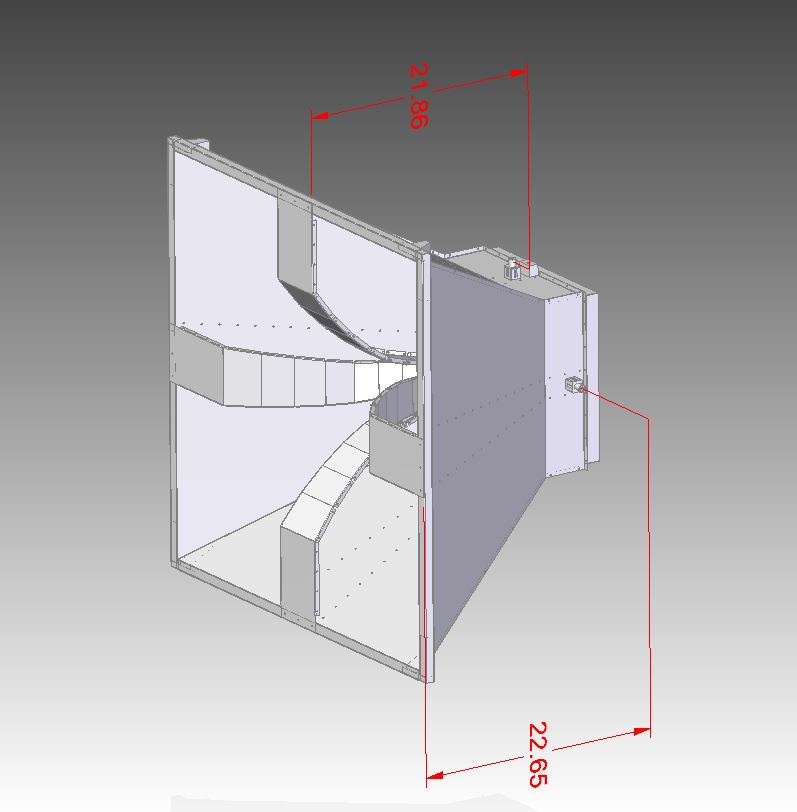
\includegraphics[width=0.7\textwidth]{ANITA_HORN_FEED_DIM}
	\caption{CAD model of the Seavey quad ridge horn antenna.  The distance between the face of the antenna and the feed point is annotated for use in estimating the phase center location as a function of frequency.\cite{Christian}}
\label{fig:antDim}
\end{figure}



If the antennas are identical, i.e $\mathcal{H}_{Rx}(f) = \mathcal{H}_{Tx}(f)$, Equation \ref{eqn:antHeight} becomes:

\begin{gather*}
\mathcal{H}_{ant}(f) = \sqrt{ \frac{c r(f)}{if} \frac{\mathcal{F}_{rec}(f)}{\mathcal{F}_{src}(f)} } \\
\label{eqn:antHeight2}
\end{gather*}

Note that using Equation \ref{eqn:antHeight2} results in a sign degeneracy, as there are two possible solutions that satisfy the square root term.  This manifests itself as a lack of constraint on the absolute polarity of the emitted signal.  Determining the absolute polarity of the antennas requires using a calibrated reference antenna of which the polarity is previously known.


Complex antenna height relates electric field to measured voltage according to the following equation:

\begin{equation}
\frac{V_{rec}(t)}{\sqrt{Z_{sys}}} = h(t) \circ \frac{ E_{rad}(t) }{ \sqrt{Z_{o}} } \\
\label{eqn:antHeight2EField}
\end{equation}

Where $\circ$ is the convolution operator, $Z_{sys}$ is the matched impedance of the transmission line (50$\Omega$ in our system) and $Z_{o}$ is the impedance of free space (377$\Omega$).  Using these relationships it is possible to solve for the conversion between electric field and induced voltage.


	\subsection{Antenna Gain}
		The figure of merit for the absolute radiative power of an an antenna is called the Antenna Gain, and is calculated by taking the logaritm of the ratio between the measured peak radiated power of the antenna under test and that of an isotropically emitting antenna.  This value takes on the units dBi.  The equation to determine the antenna gain from the normalized complex antenna height is shown in Equation \ref{eqn:antGain2}.
		
\begin{equation}
G_{eff}(f) =  \frac{4\pi f^{2}}{c^{2}} | \mathcal{H}_{ant}(f)|^{2}
\label{eqn:antGain2}
\end{equation}

	\subsection{Results of Palestine Antenna Measurements}
	
		All 48 antennas for the ANITA3 flight were measured at the Columbia Scientific Balloon Facility (CSBF) in Palestine, TX during the 2014 integration campaign.  The complex antenna height did not noticably vary between antennas, and resulted in an average antenna gain of approximately 10dBi.  Figures \ref{fig:antennaGain} through \ref{fig:antResponse_fftV} show the results for all antennas.
		

\begin{figure}
\centering
	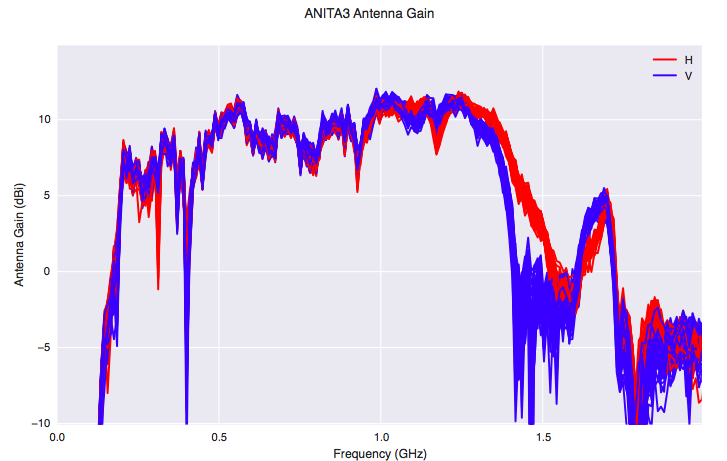
\includegraphics[width=\textwidth]{antennaGain}
	\caption{Results for the antenna gain as a function of frequency for all 48 ANITA3 horn antennas.}
\label{fig:antennaGain}
\end{figure}

\begin{figure}
\centering
	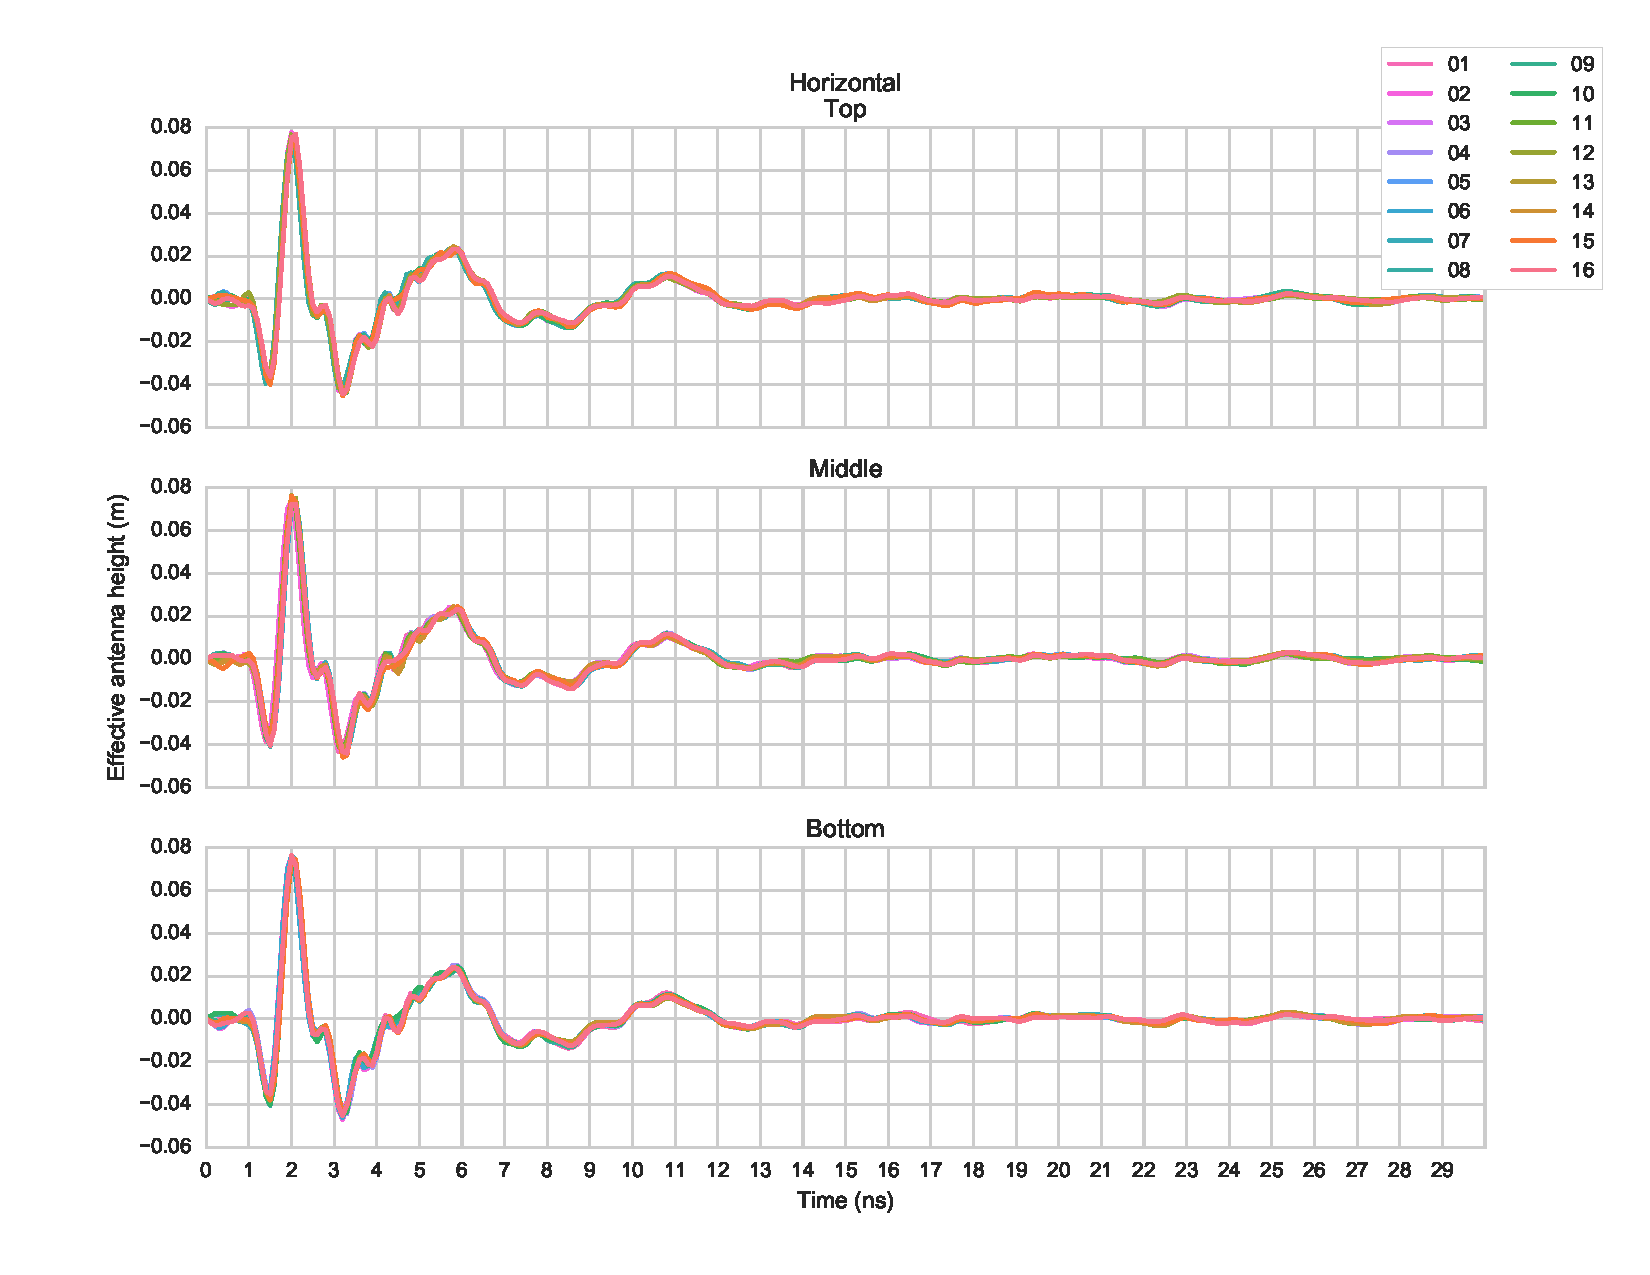
\includegraphics[width=\textwidth]{antResponse_timeH}
	\caption{Time domain impulse response of the horizontally oriented polarizations of the ANITA3 horn antennas.}
\label{fig:antResponse_timeH}
\end{figure}

\begin{figure}
\centering
	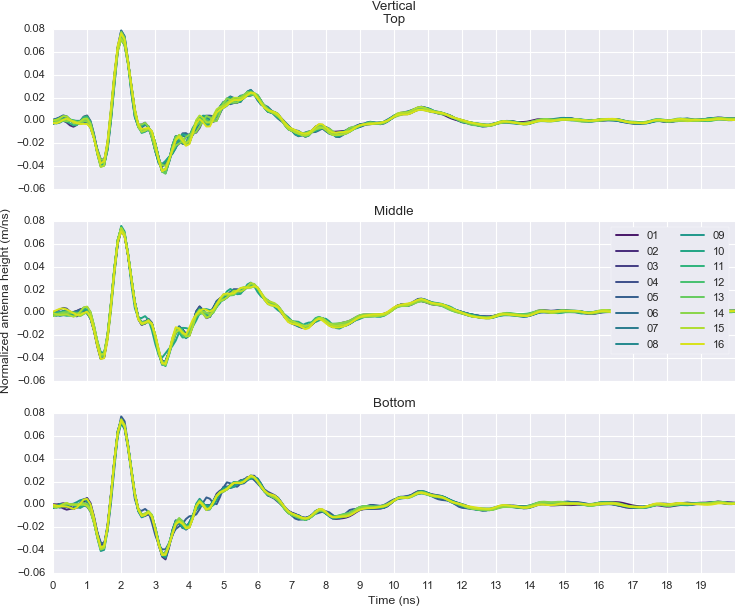
\includegraphics[width=\textwidth]{antResponse_timeV}
	\caption{Time domain impulse response of the vertically oriented polarizations of the ANITA3 horn antennas.}
\label{fig:antResponse_timeV}
\end{figure}

\begin{figure}
\centering
	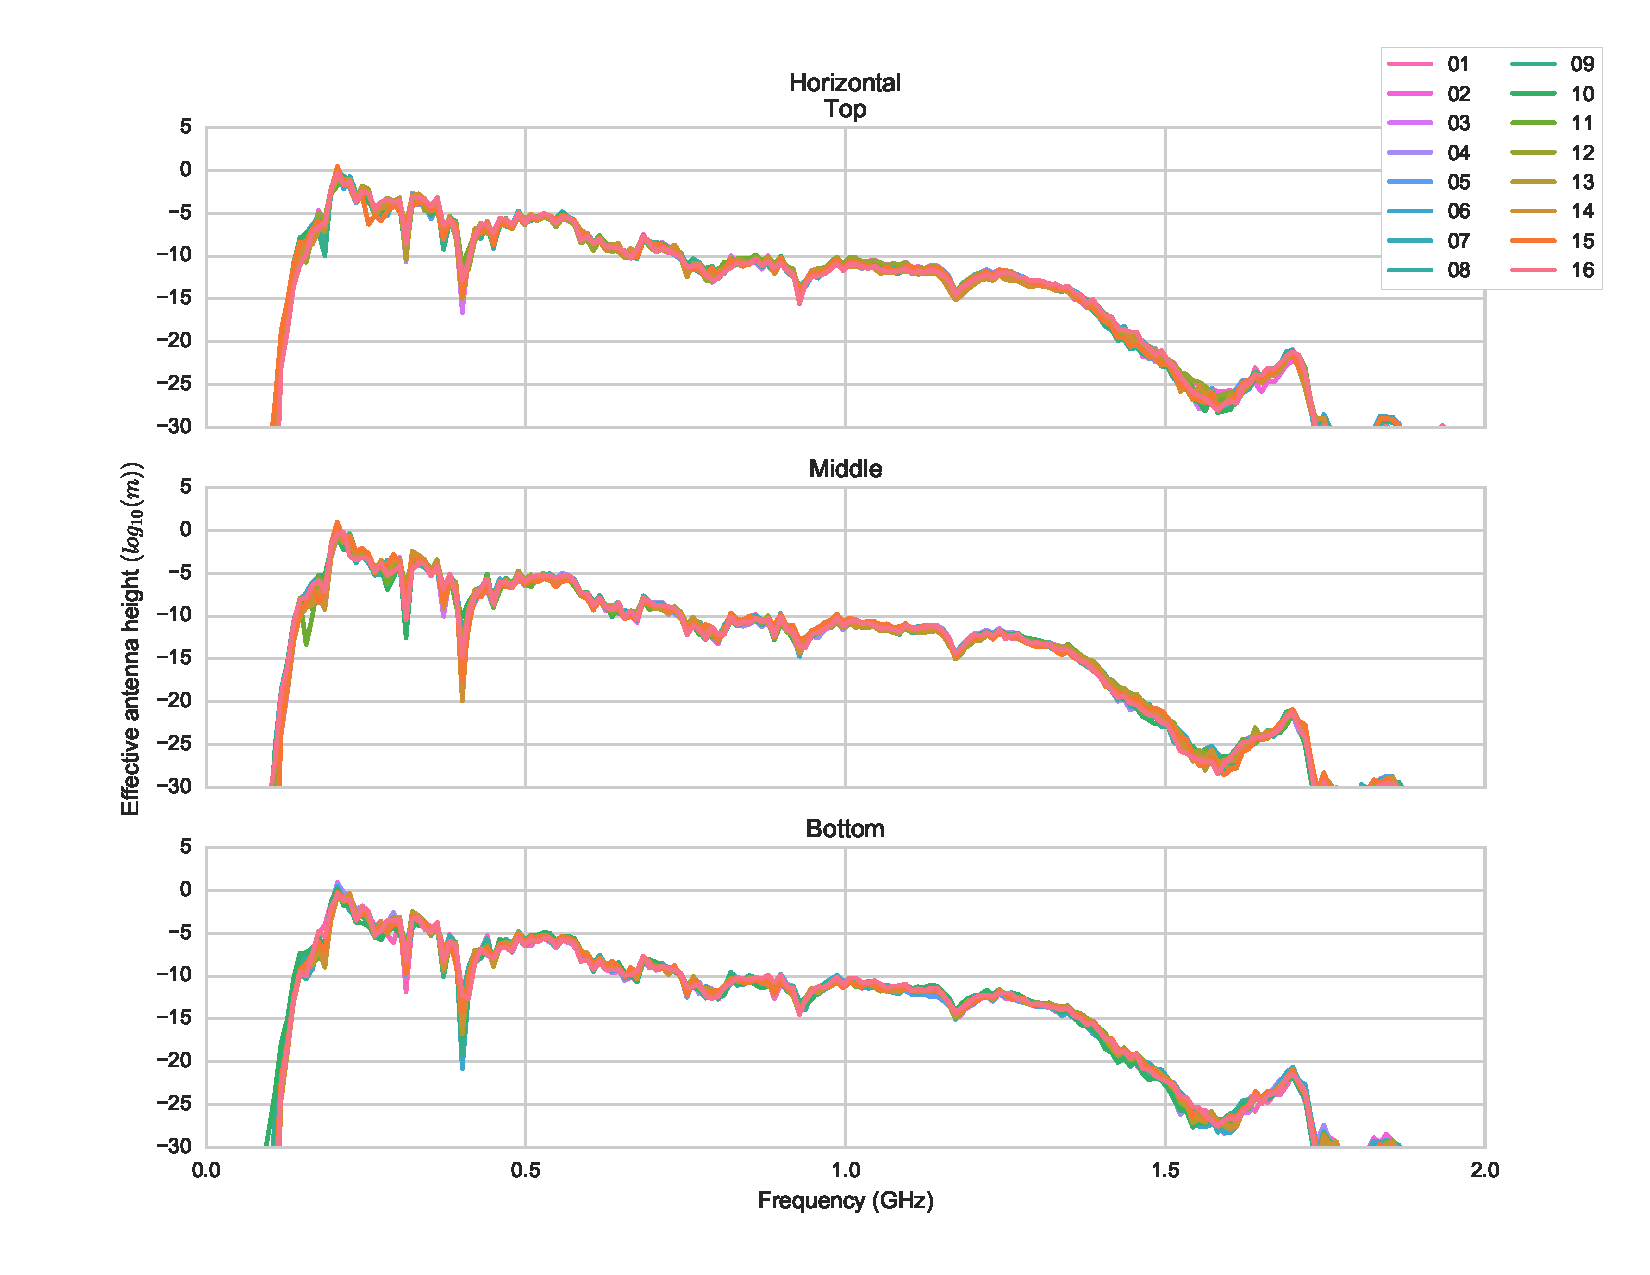
\includegraphics[width=\textwidth]{antResponse_fftH}
	\caption{Complex antenna height for the horizontally oriented polarizations of the ANITA3 horn antennas.}
\label{fig:antResponse_fftH}
\end{figure}

\begin{figure}
\centering
	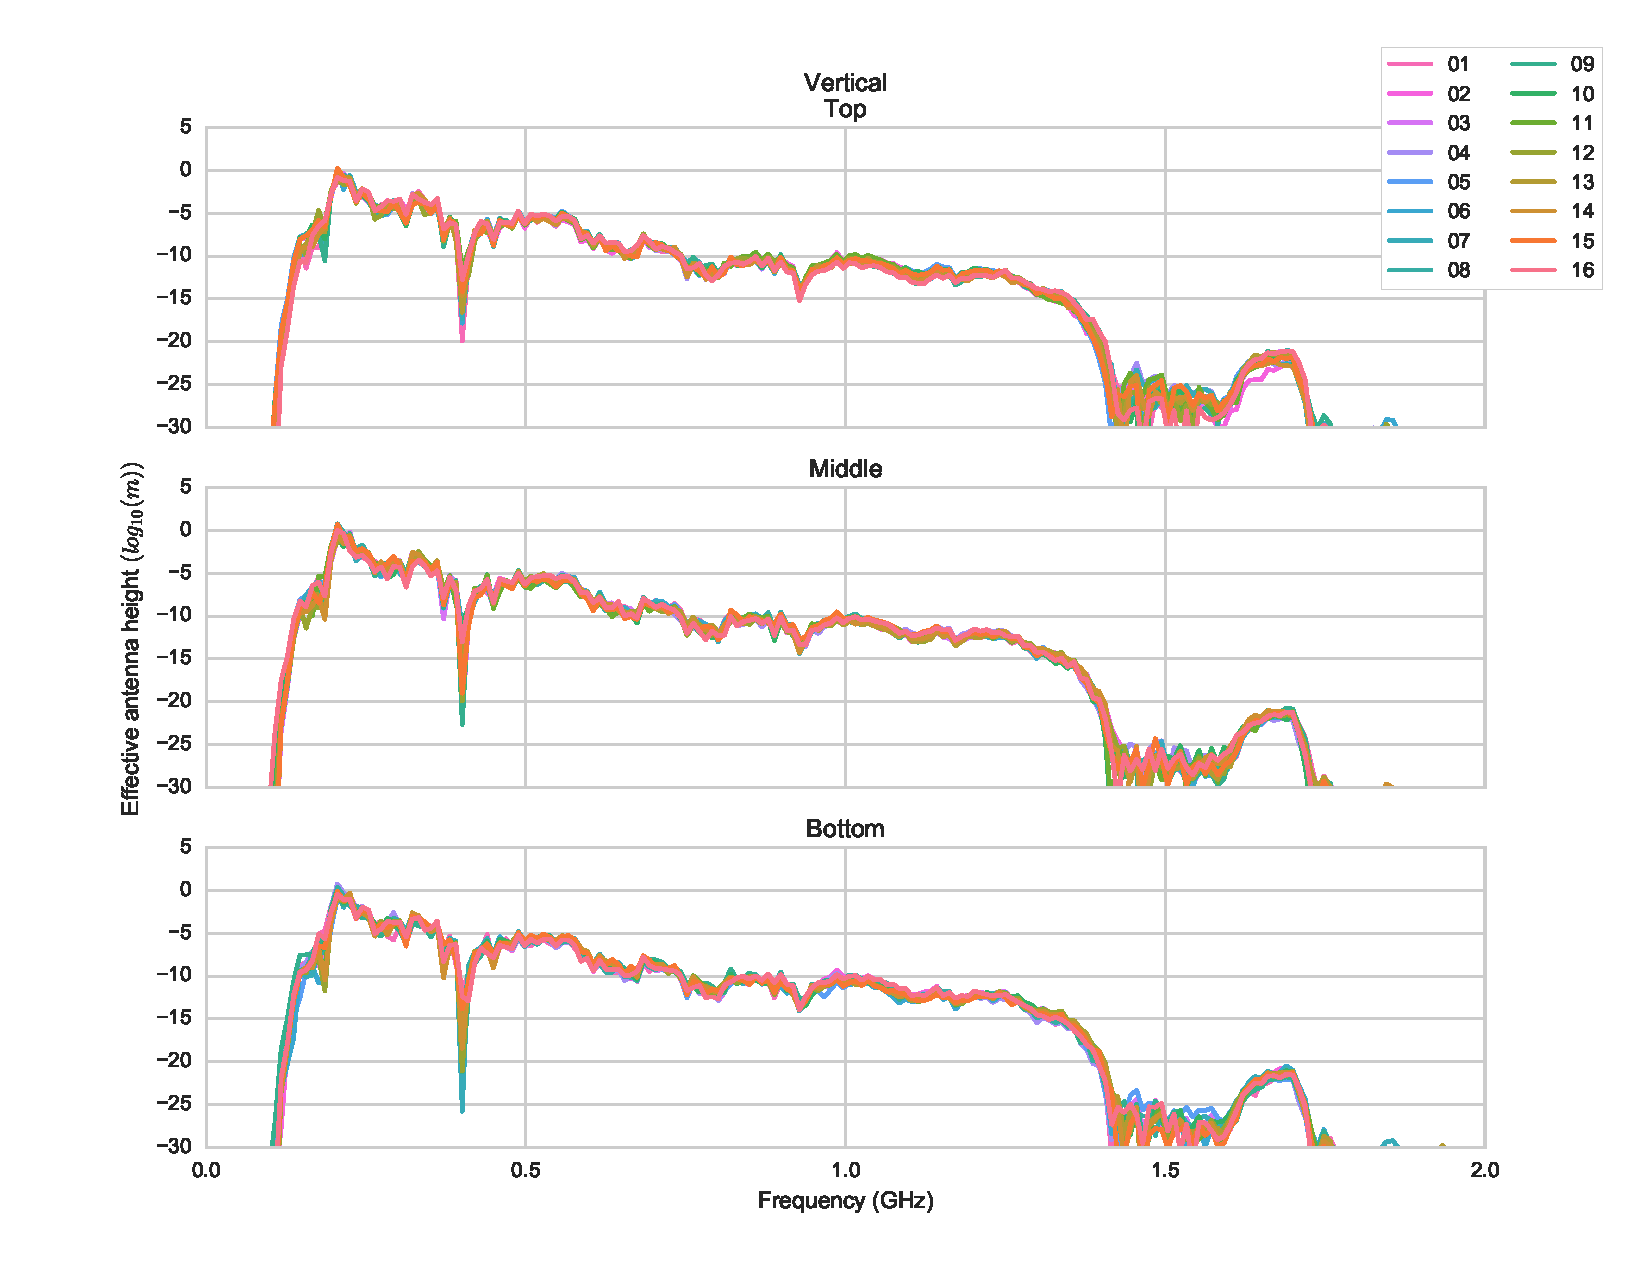
\includegraphics[width=\textwidth]{antResponse_fftV}
	\caption{Complex antenna height for the vertically oriented polarizations of the ANITA3 horn antennas.}
\label{fig:antResponse_fftV}
\end{figure}


%	\subsection{Comparison of Different Measurements}
%	 	Measurements of the antennas were taken in multiple configurations since their initial batch purchase in 2012.  To determine the validity and repeatability of the measurements, I compared the consistency between the three calculated boresight antenna heights and the manufacturing specified antenna height provided by Seavey.


	\subsection{Off Angle Antenna Response}
		An additional characteristic of the antennas is their response to signals that are incident on the antenna at angles off the boresight.  Seavey provided manufacturing test result plots for the off angle response at five discrete frequencies.  These were manually digitized and replotted, and are presented in Figure \ref{fig:seaveyOffAngle}.
		
		
\begin{figure}
\centering
	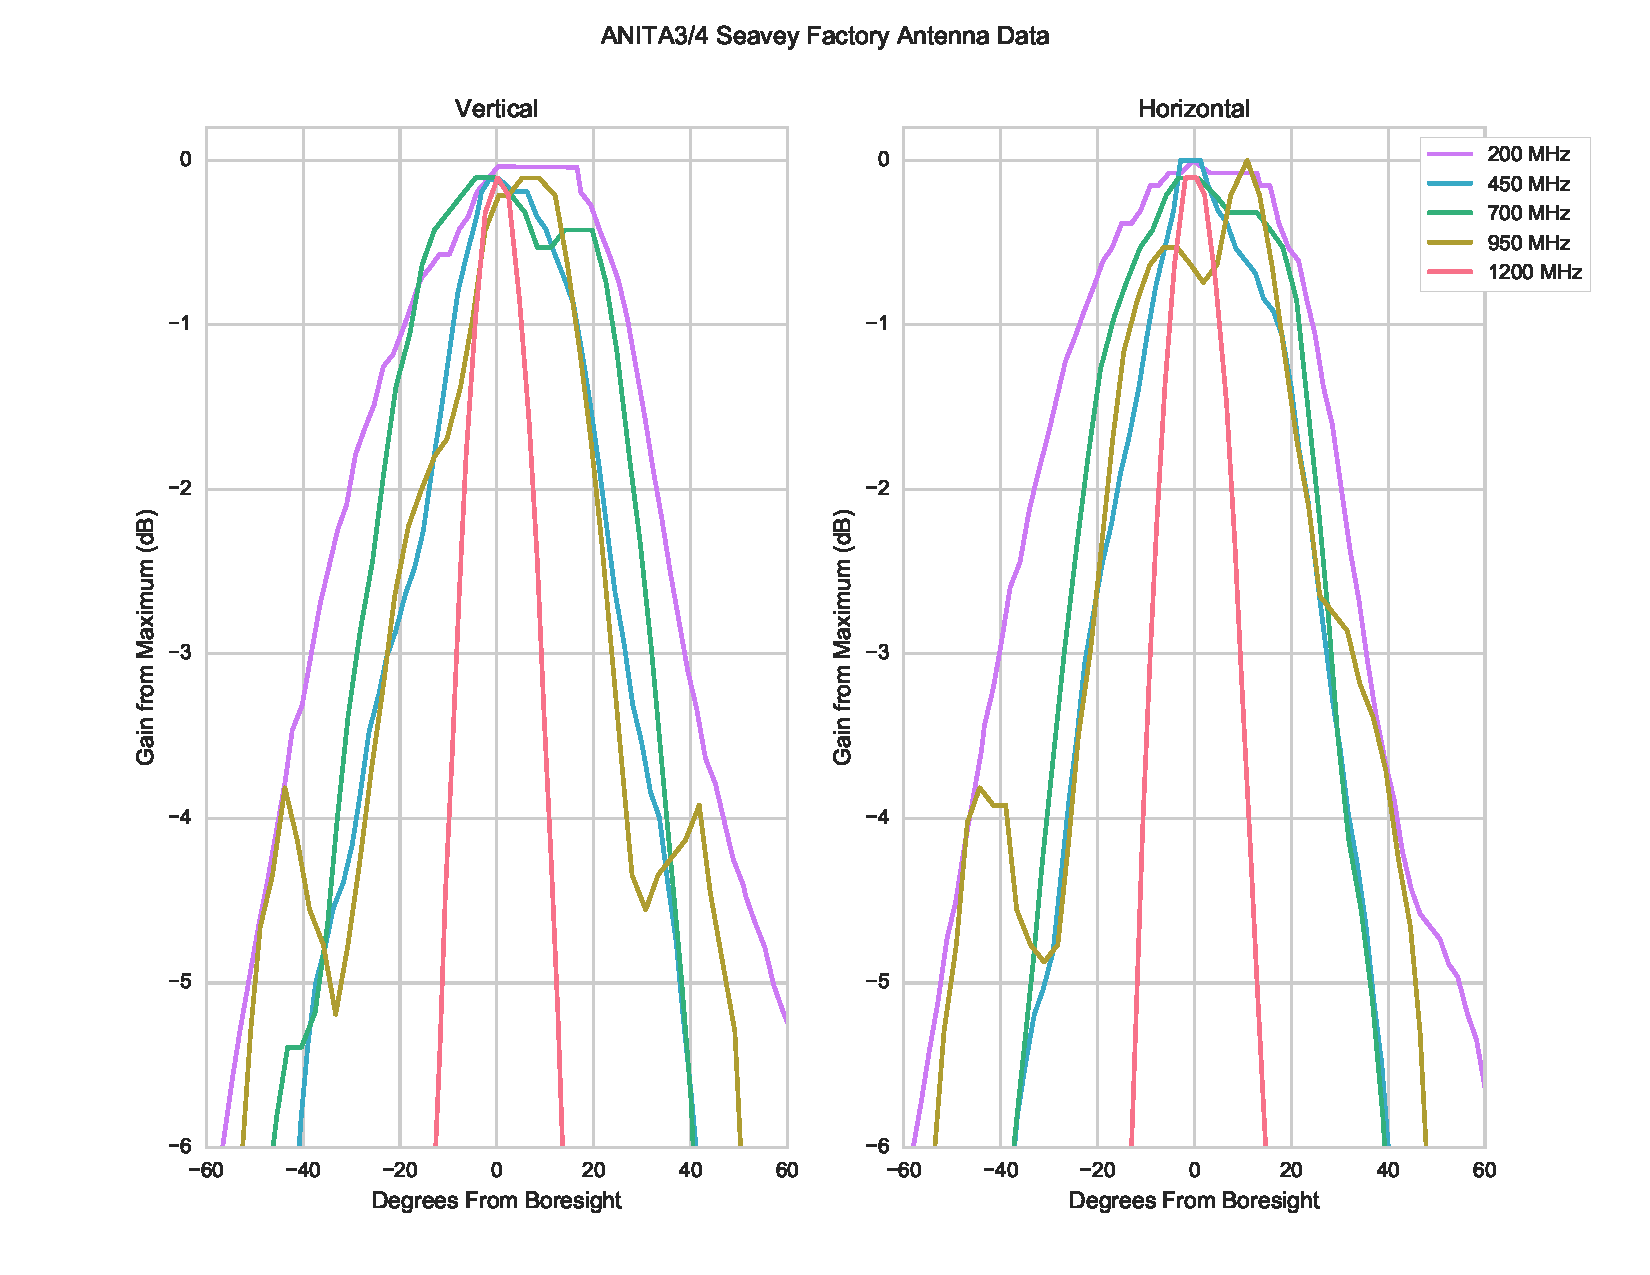
\includegraphics[width=\textwidth]{seaveyDataPlotter}
	\caption{Replotted off angle antenna responses received from Seavey after antenna manufacturing.  Gains are referenced to the maximum received power, which is not required to be the boresight angle.  Responses are in reference to the electric field incident on the respective polarization ridge of the antenna.}
\label{fig:seaveyOffAngle}
\end{figure}

	\subsubsection{Off Angle Antenna Measurement} %this actually doesn't really work
To independently measure the off angle response of the antennas, the UH anechoic chamber data was used, despite its low frequency near field limitations.  The above procedure for developing complex antenna height was done for multiple rotation angles of the receive antenna while the transmission antenna was kept stationary.  Because of this, Equation \ref{eqn:antHeight} must be used with $\mathcal{H}_{TX}(f)$ set as the average complex antenna height measured wile the antennas were in the zero rotation angle configuration.  Cables and propagation losses are removed from the measurement. The results of this analysis are shown in Figures \ref{fig:chamberHpol} and \ref{fig:chamberVpol}.
		
\begin{figure}
\centering
	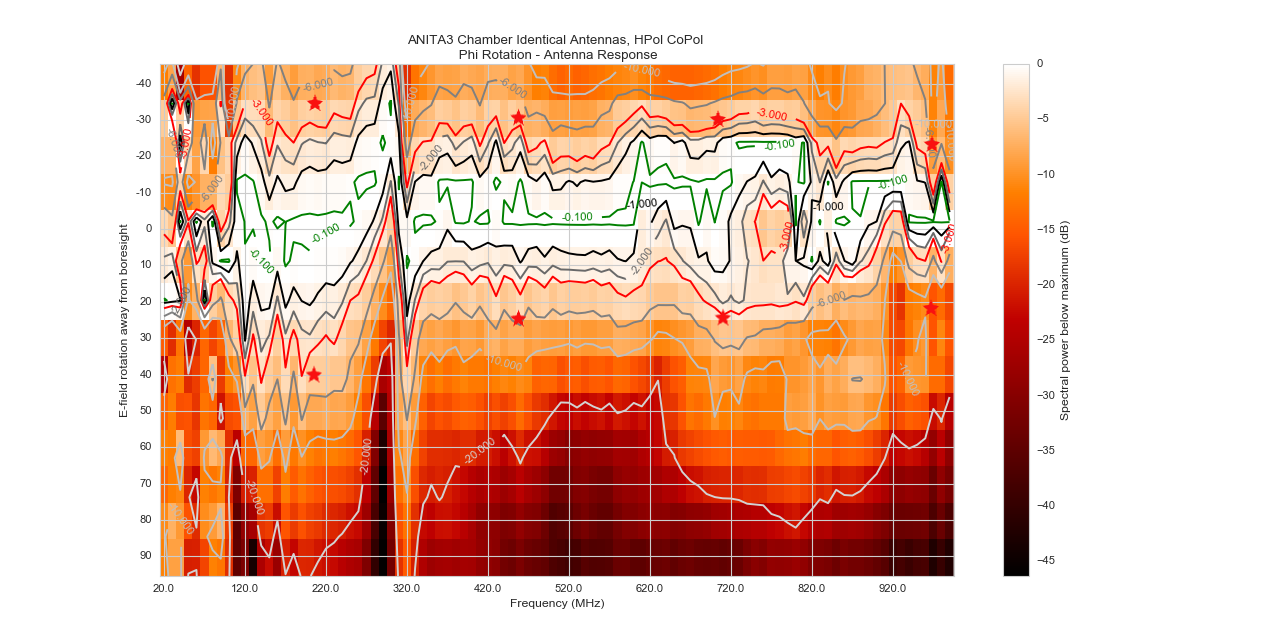
\includegraphics[width=\textwidth]{ANITA3Chamber_HPol_Phi_S21}
	\caption{Off angle antenna gains from the analysis of the Seavey horn antennas for the E-field of the Horizontally polarized ridge, rotated horizontally.  This corresponds to the azimuthal response for the Hpol channels of the ANITAIII instrument.  Measurements were taken in the UH anechoic chamber with identical receive and transmit antennas, with only the receive antenna being rotated.  Counter-clockwise rotation beyond 45$^\circ$ is obstructed by the chamber wall.  Red stars denote the -3dB points from the Seavey manufacturing data at the frequencies measured by them. A ``wandering'' of the beam pattern caused by the Vpol feed structure can be seen at 320MHz.}
\label{fig:chamberHpol}
\end{figure}

\begin{figure}
\centering
	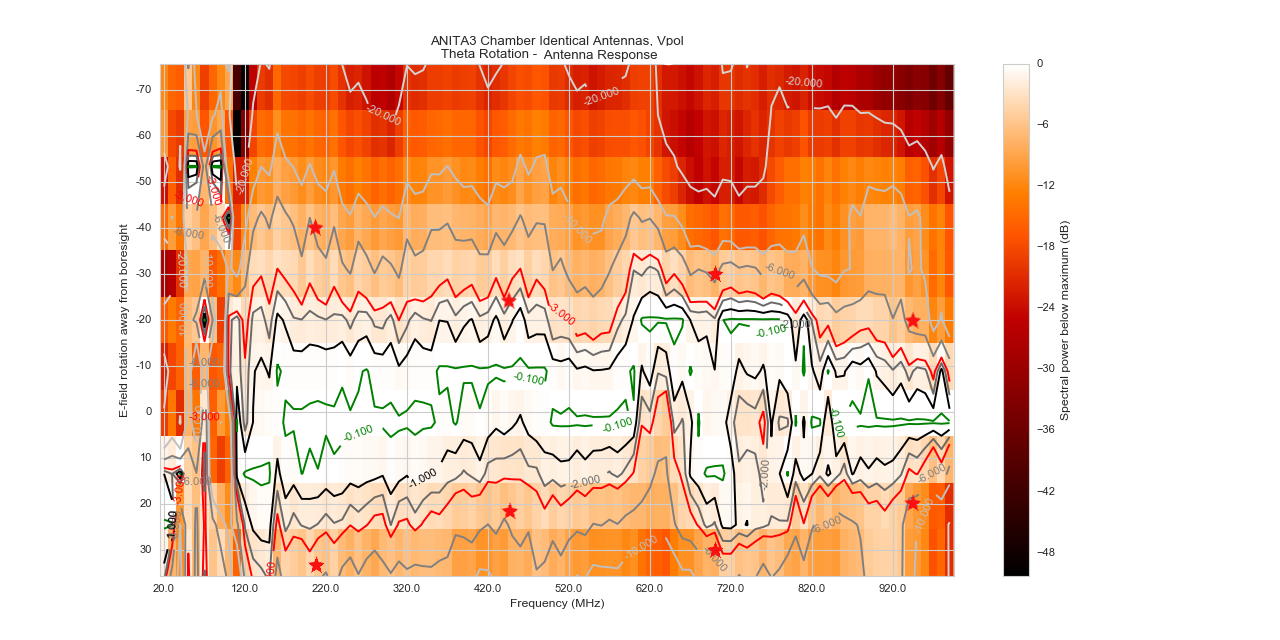
\includegraphics[width=\textwidth]{ANITA3Chamber_VPol_Theta_S21}
	\caption{Off angle antenna gains from the analysis of the Seavey horn antennas for the E-field of the Vertically polarized ridge, rotated vertically.  This corresponds to the elevation response for the Vpol channels of the ANITAIII instrument.  Measurements were taken in the UH anechoic chamber with identical receive and transmit antennas, with only the receive antenna being rotated.  Downward rotation beyond 35$^\circ$ is obstructed by the chamber floor.  Red stars denote the -3dB points from the Seavey manufacturing data at the frequencies measured by them.}
\label{fig:chamberVpol}
\end{figure}


Th


%%%%%%%%%%%%%%%%%%%%%%%%%%%%%%%%%%%%%%%%%%%
\section{RF Signal Chain Impulse Response}
		
	\subsection{Measurements Summary}
		Complex phasor response measurements for each of the 96 signal chains flown in the ANITA3 instrument were taken in Antarctica immediately preceding the flight. A broad band impulse was injected into each channel sequentially and measured by the on board flight electronics.  This signal was split at the source and simultaneously measured by an oscilloscope, providing an input and output reference signal which we can compare to determine the full complex transfer function.  A diagram of the setup is seen in Figure \ref{fig:sigChainSetup}.


\begin{figure}
	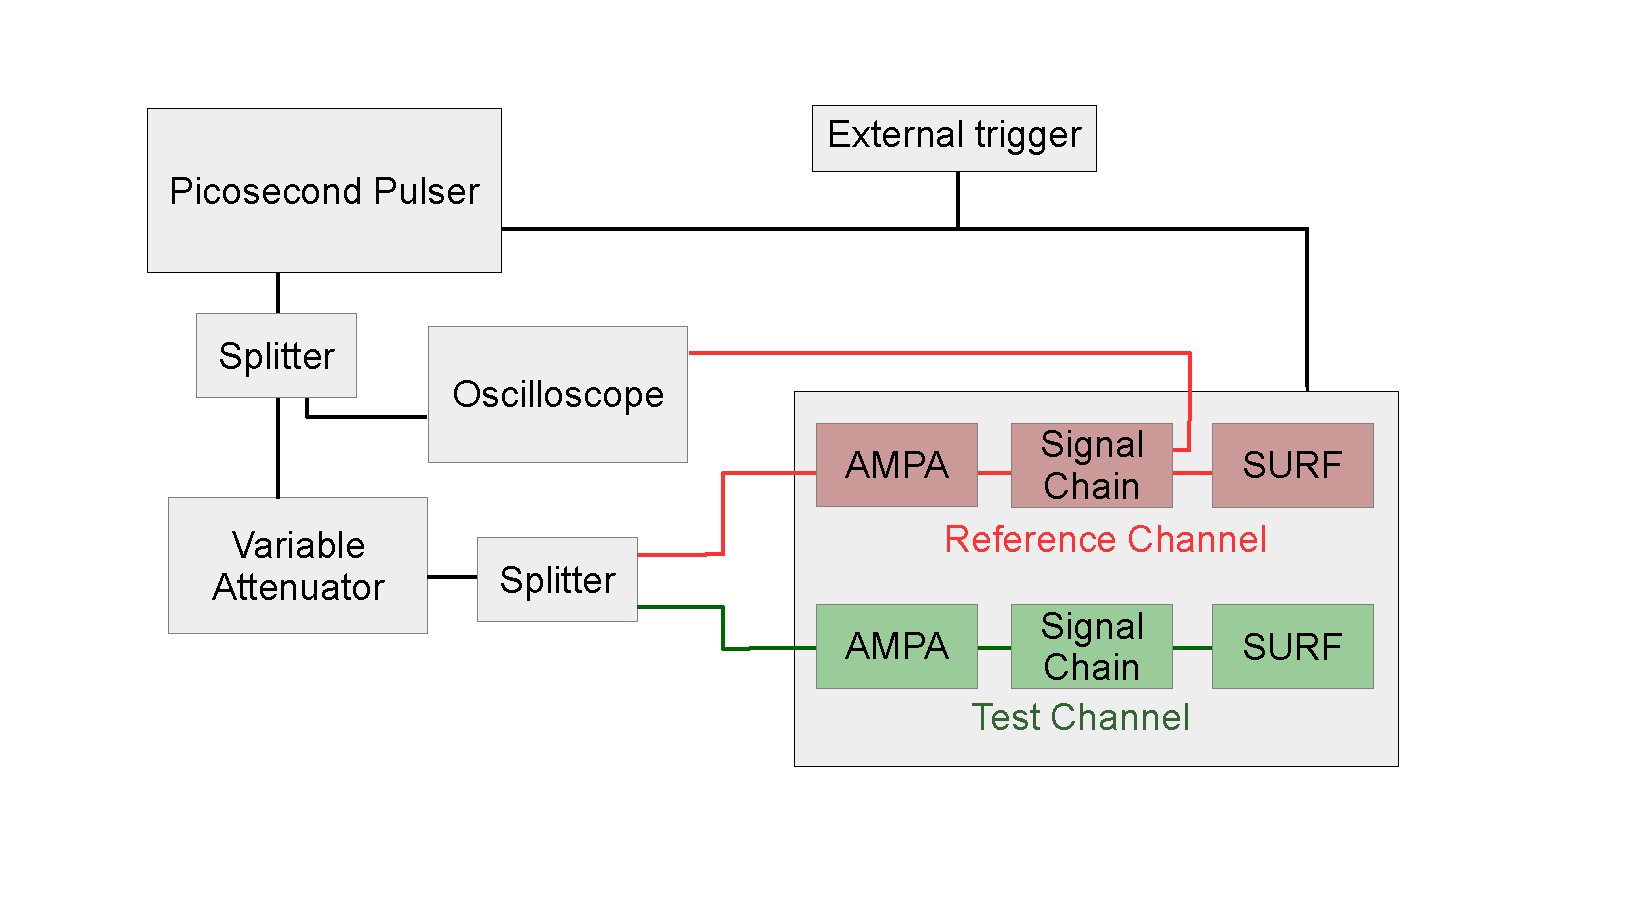
\includegraphics[width=\textwidth]{antarctica14_calSetup}
	\caption{A schematic of the pulse insertion calibration setup used immediately before flight with the full signal chain in Antarctica in 2014}
	\label{fig:sigChainSetup}
\end{figure}
			
	Note that the cables connecting the various elements of the calibration test setup are not present in the final flight configuration, and needed to be separately measured and removed.
			

		
	\subsection{Complex Transfer Function}
		The full mathematical relationship between two waveforms that have traversed a non-linear signal network is called the complex transfer function, which I will denote with $h_{sig}(t)$ and its Fourier transform equivalent $\mathcal{H}_{sig}(f)$.  The relationships between a measured input signal $V_{in}(t)$ and output signal $V_{out}(t)$, and their respective Fourier transform equivalents $\mathcal{F}_{in}(f)$ and $\mathcal{F}_{out}(f)$, are shown in Equation \ref{eqn:ComplexTF}.
	
\begin{equation}
\begin{split}
V_{out}(t) = h_{sig}(t) \circ V_{in}(t) \\
\mathcal{F}_{out}(f) = \mathcal{H}_{sig}(f) \mathcal{F}_{in}(f) \\
\label{eqn:ComplexTF}
\end{split}
\end{equation}

The $\circ$ denotes a convolution operator.  The Fourier domain equivalent to convolution is complex multiplication, which can be seen in this equation pair.  Using these equations and the measurements of input and output digitized time domain waveforms we can determine the complex transfer function for each channel of the ANITA3 signal chain.


	\subsection{Methodology}
		The input and output waveforms were recorded by different devices with different sampling rates and record lengths, and so some digital processing must be done to make them directly relatable.  The oscilloscope's 10GS/s (100ps/sample) digitized readout of the input pulse waveform was treated as the sampling rate reference for this analysis.  The record length was chosen to be 1024 samples which allows for a 102.4ns window, comparable to the nominal window size of the LABRADOR.
		
		The LABRADOR returns unevenly sampled waveforms at a nominal 2.6GS/s (385ps/sample) rate.  To compare the two signals, first an Akima piecewise cubic spline was applied to determine an equivalent evenly sampled waveform.  This waveform was either zero padded or cut in order to make the number of points equal to 256.  Next, the Fourier equivalent series, which has $\frac{N}{2}+1 = 129$ samples was found. This was zero padded by a factor of $\frac{dT_{old}}{dT_{new}}*N_{\mathcal{H}} = \frac{384ps}{100ps}*129$, up to 496 samples.  Taking the inverse Fourier transform of this zero padded series results in an up-sampled time domain waveform at 10GS/s.  An example of this up-sampling is shown in Figure \ref{fig:sigChain_upsample}.
		
\begin{figure}
\centering
	\includegraphics[width=\textwidth]{sigChain_upsample}
	\caption{An example from channel 01BH of even resampling and up-sampling the original unevenly sampled LABRADOR digital readout.  The peak of the impulse is shown zoomed, while a view of the entire waveform can be seen in the inset frame showing the macro-consistency of the methods.  The method used in this analysis is  FFT up-sampling.  Despite undershooting some points, it minimally distorts the spectral power and phase response of the signal.}
\label{fig:sigChain_upsample}
\end{figure}			
		
		After the input and output time domain waveforms had the same waveform characteristics, they were separately correlated and averaged to reduce thermal and electronic noise introduced by the system.  The pulse captured by the oscilloscope underwent no amplification and had an extremely high signal to noise ratio, and this averaging was done primarily to equivalently sample the interval over which output pulse data would be averaged.  However, the signal chain's high gain specification, required for detection of the physics phenomenon under test, necessitated significant attenuation of the signal prior to it being fed into the front of the chain.  This lowered the signal to a level only moderately above the electronic noise introduced by the first stage amplifiers and room temperature thermal noise present in the attenuator and cables.  This allowed real physics signals to fall within the dynamic range of the digitizer.  Aligning and averaging reduces the noise contribution by $\sqrt{N}$, leaving primarily the signal.  The number of averages in this analysis for all waveforms was $N=1024$.  An example of the reduction of noise is seen in Figure \ref{fig:sigChain_noiseReduction}.
		
\begin{figure}
\centering
	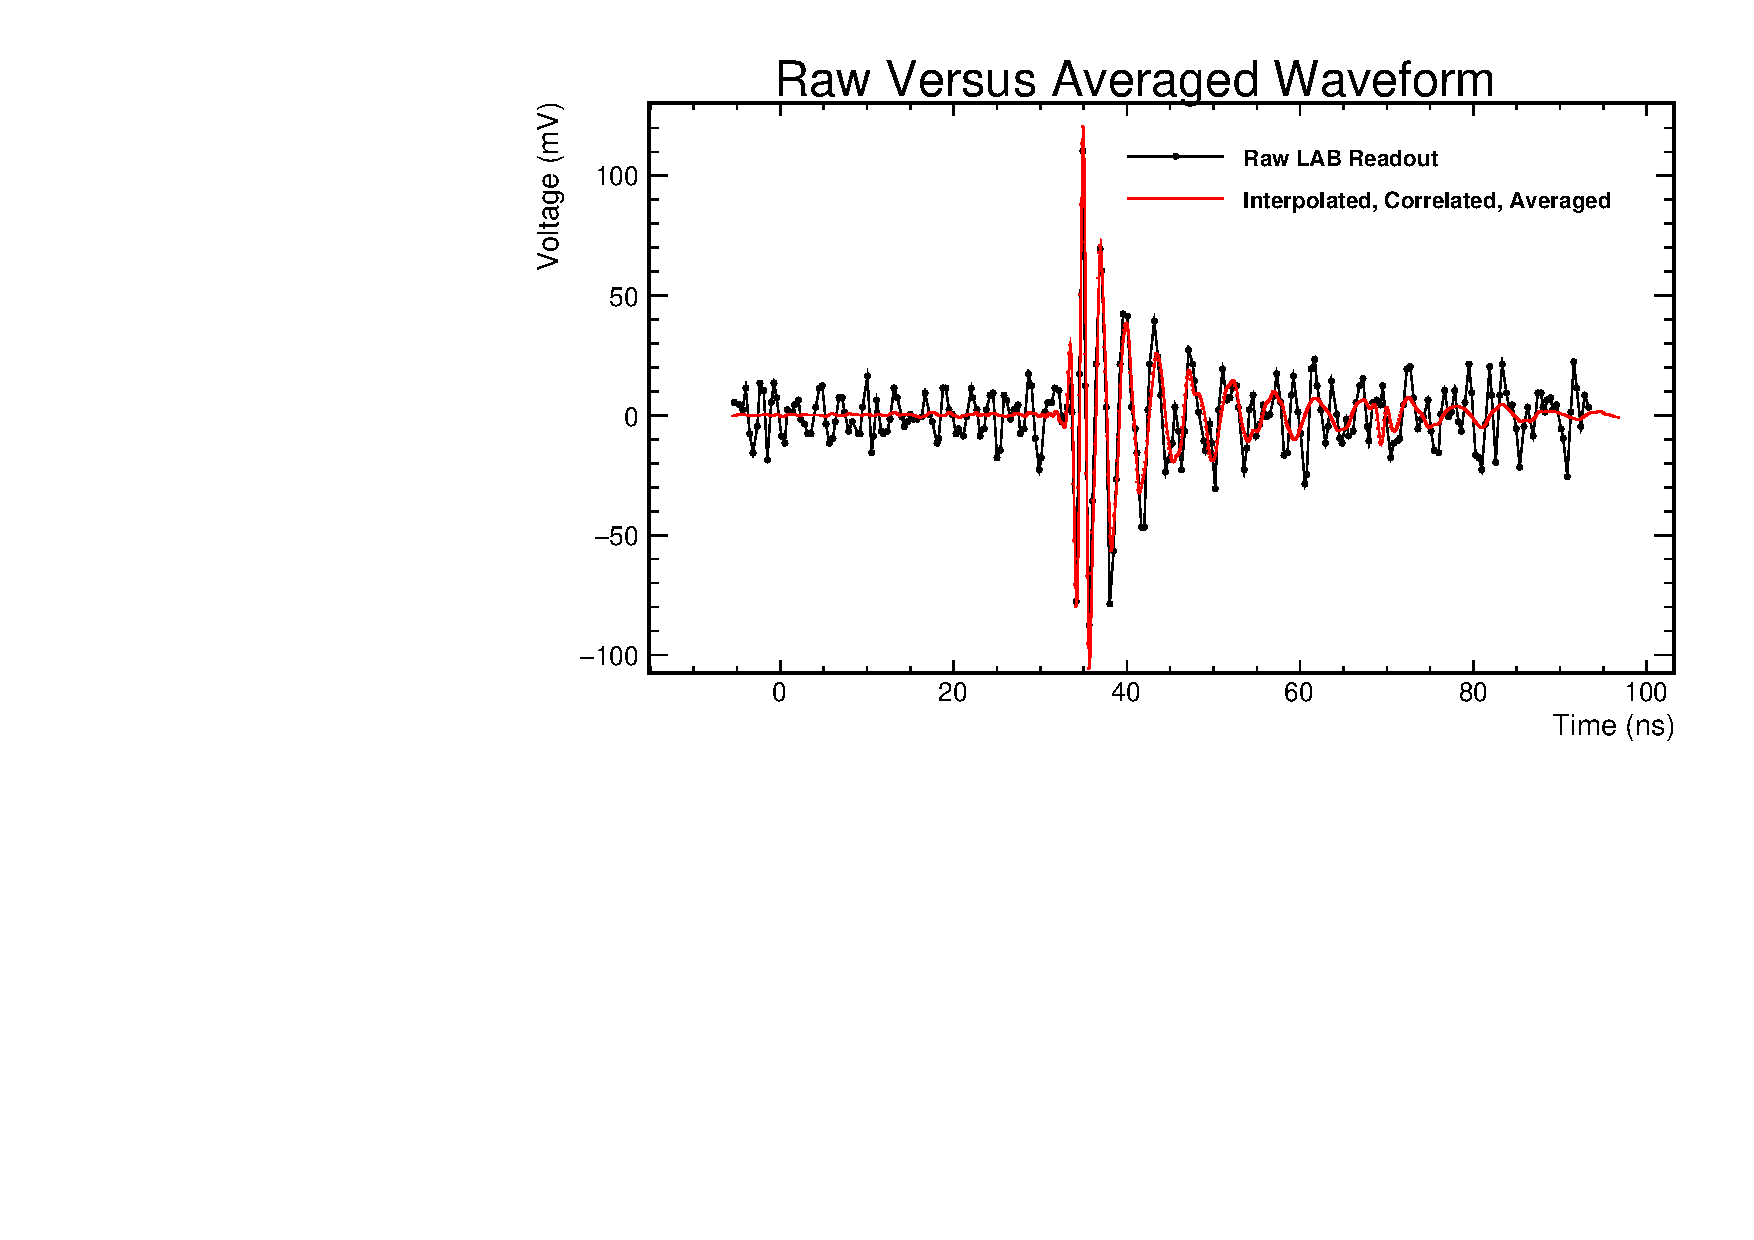
\includegraphics[width=\textwidth]{sigChain_noiseReduction}
	\caption{An example from channel 01BH of the reduction in individually sampled waveform thermal and electronic noise versus the correlated and averaged signal result.}
\label{fig:sigChain_noiseReduction}
\end{figure}	
		
		The units of the signal digitized by the oscilloscope have been nominally calibrated by comparing the peak to peak measurement of the LAB waveform and an oscilloscope measurement taken immediately before input the the SURF , however this analysis does not use this calibration for the LABRADOR ADC conversion.  The normalized transfer function for the signal chain will include an implicit calibration of the ADC to voltage conversion.  To match units, a scaling of 1 ADC count per 1mV was used.
		
		Next, the Fourier equivalent was computed for each waveform, which was then divided to determine the transfer function for the system.  A band pass filter was placed on the resulting waveform, from 180MHz to 1.2GHz, in order to eliminate any power from regions of the spectrum not of interest.
		
		

	
	\subsection{Results for Signal Chain Transfer Function}
		The results of the analysis, separated into Vertical and Horizontally polarized channels, are presented in Figures \ref{fig:sigChain_timeH} through \ref{fig:sigChain_fftV}.  Of note are channels 05TH and 13TH.  05TH is the ALFA, a the low frequency drop down antenna that was heterodyned with a 900MHz LO and multiplexed into a digitizer.  13TH has a response slightly different than the others, mainly a higher gain at high frequencies.  This issue persisted from the ANITA3 flight to the ANITA4 flight, and the cause is unknown.
		
		
\begin{figure}
\centering
	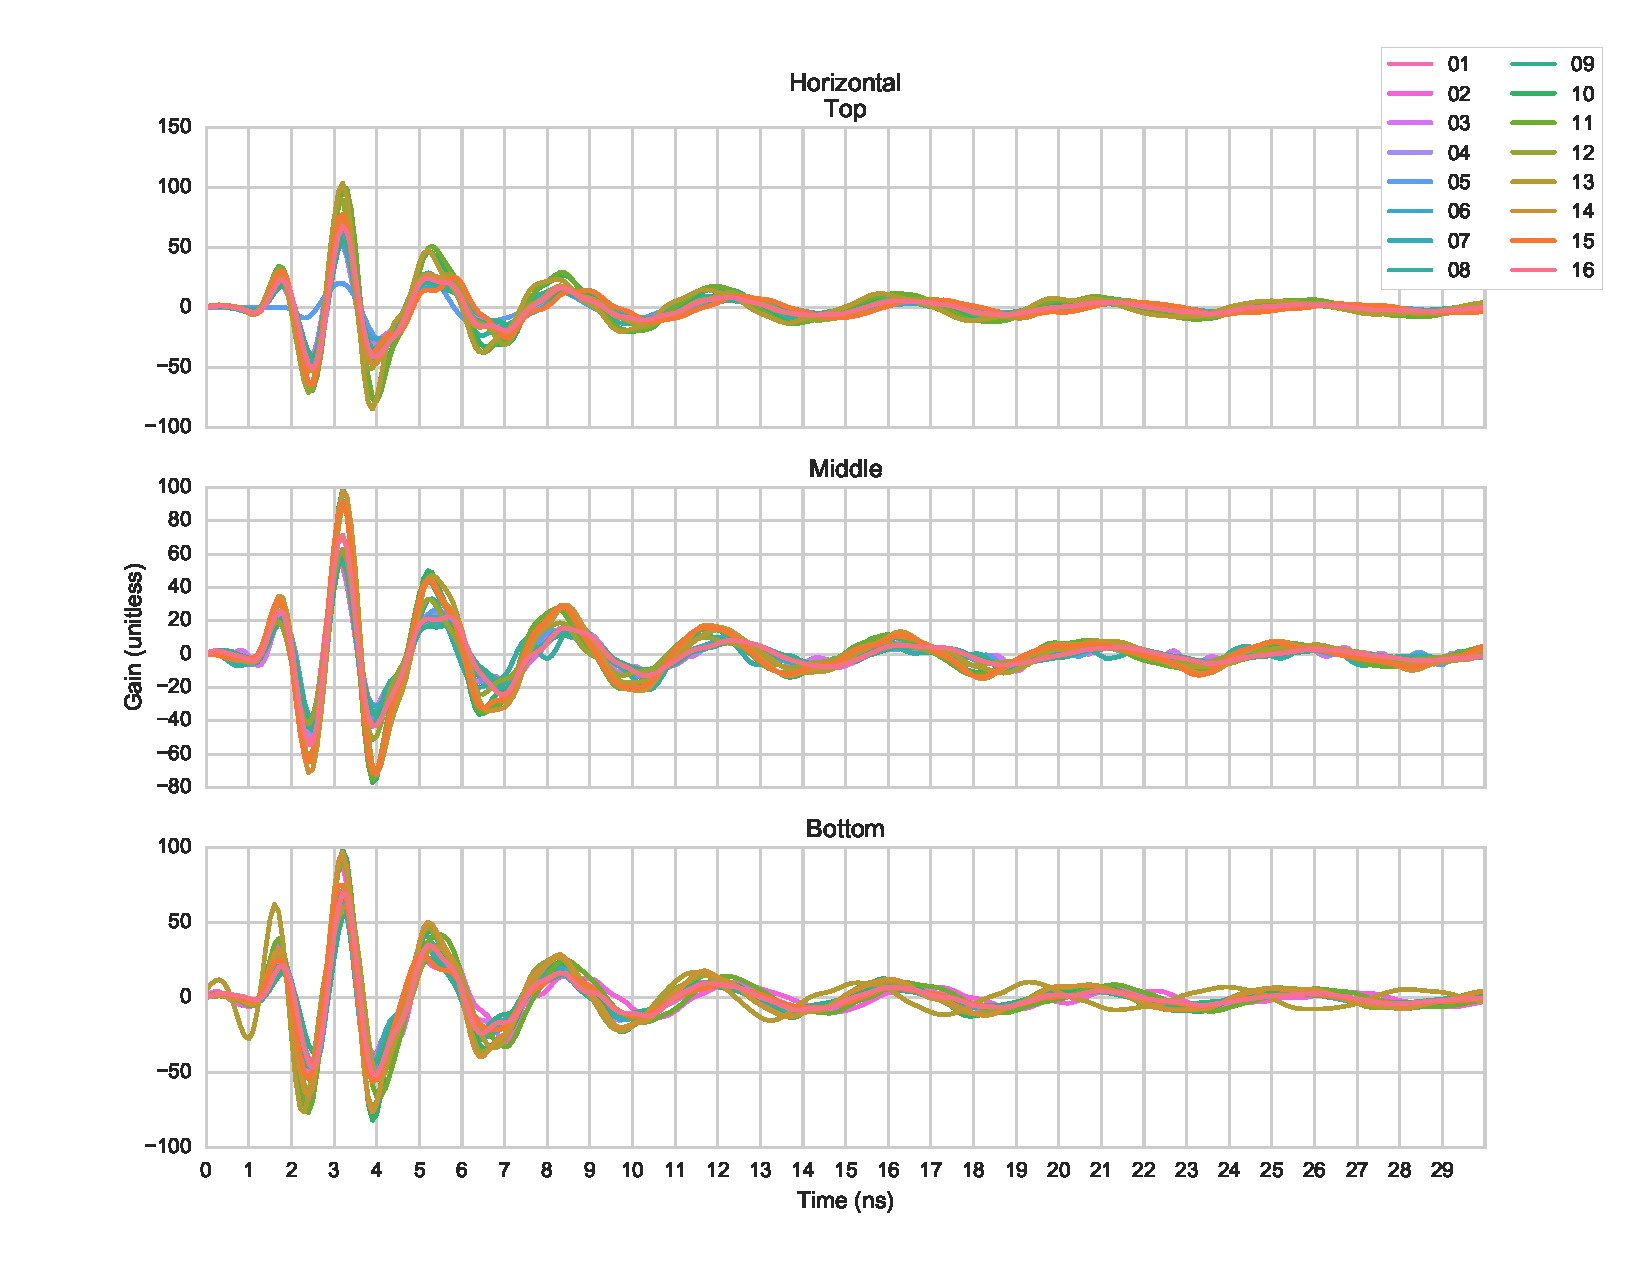
\includegraphics[width=\textwidth]{sigChain_timeH}
	\caption{Time domain impulse response of the horizontally oriented polarizations of the ANITA3 signal chain.  Note 05TH, which is the ALFA antenna, and 13BH, which has been noted has an asimilar impulse response in ANITA3 and ANITA4}
\label{fig:sigChain_timeH}
\end{figure}

\begin{figure}
\centering
	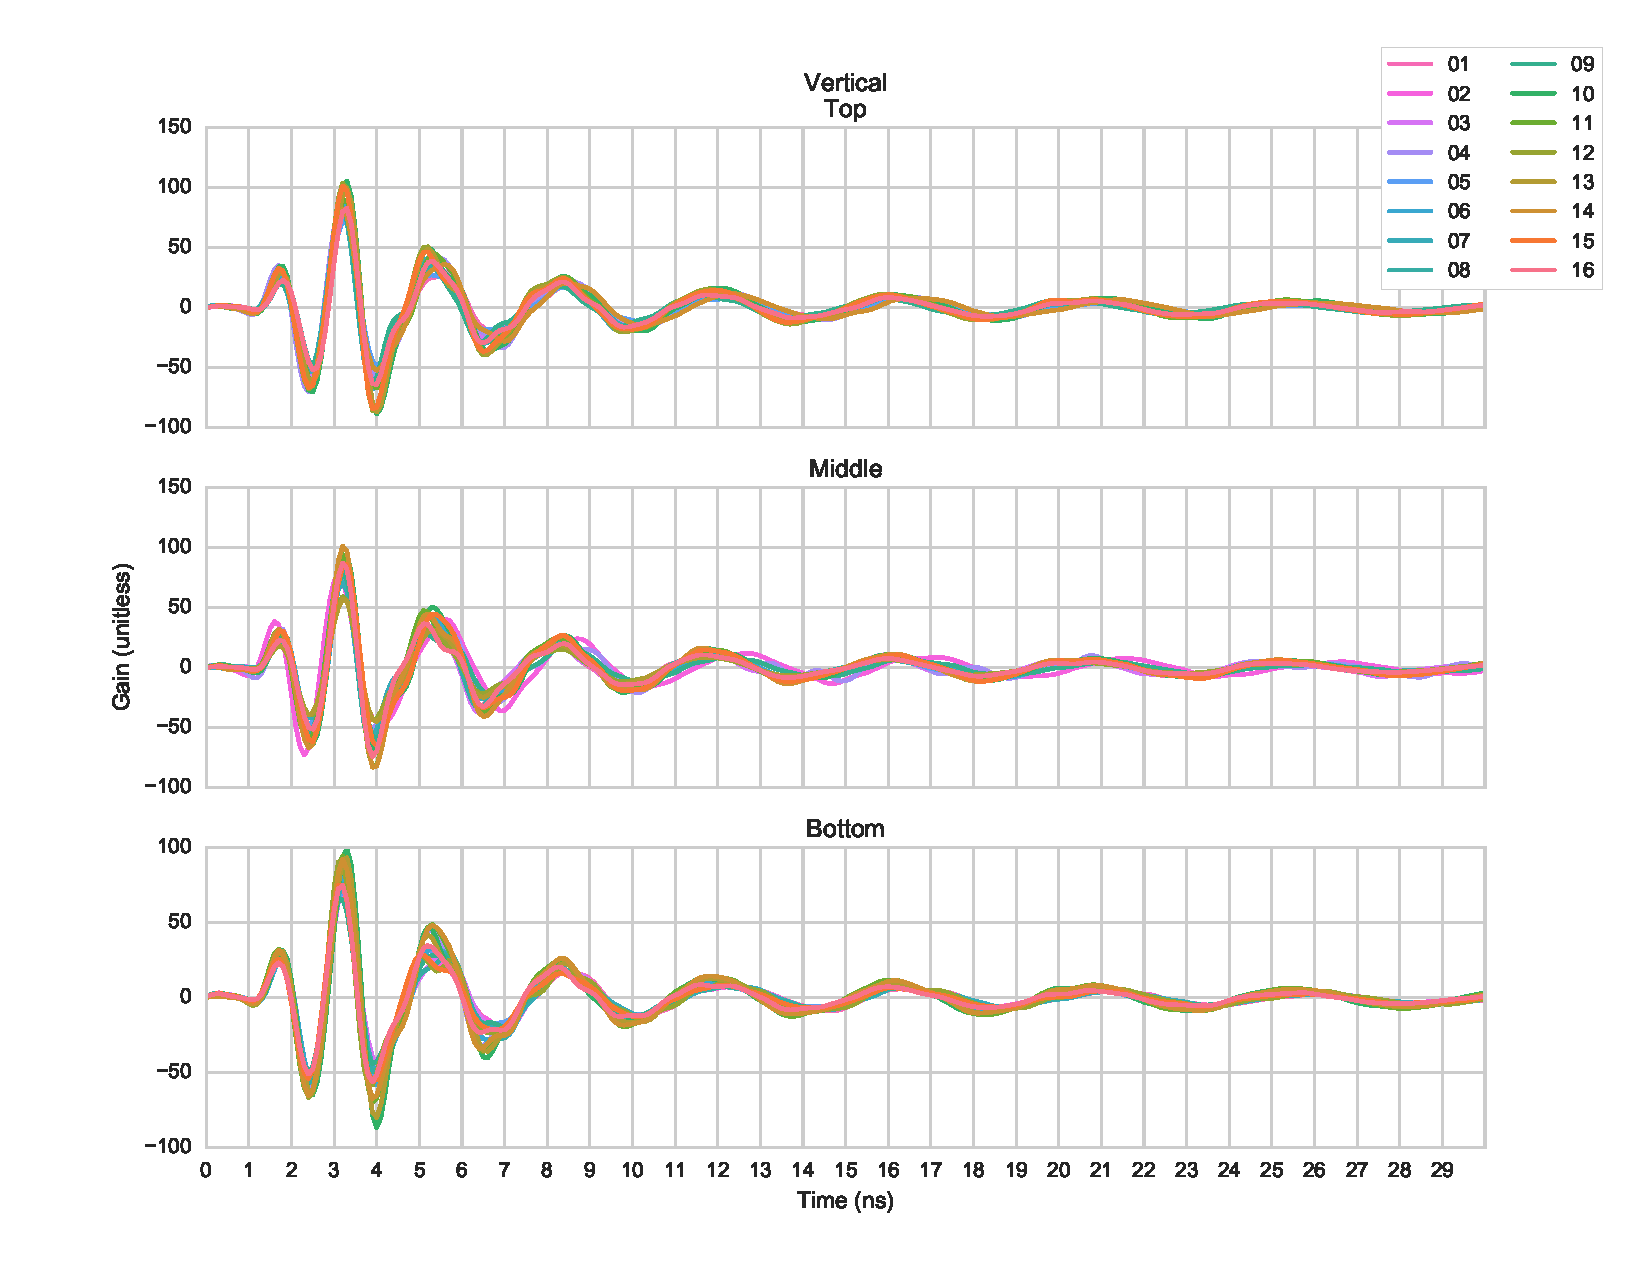
\includegraphics[width=\textwidth]{sigChain_timeV}
	\caption{Time domain impulse response of the vertically oriented polarizations of the ANITA3 signal chain.}
\label{fig:sigChain_timeV}
\end{figure}

\begin{figure}
\centering
	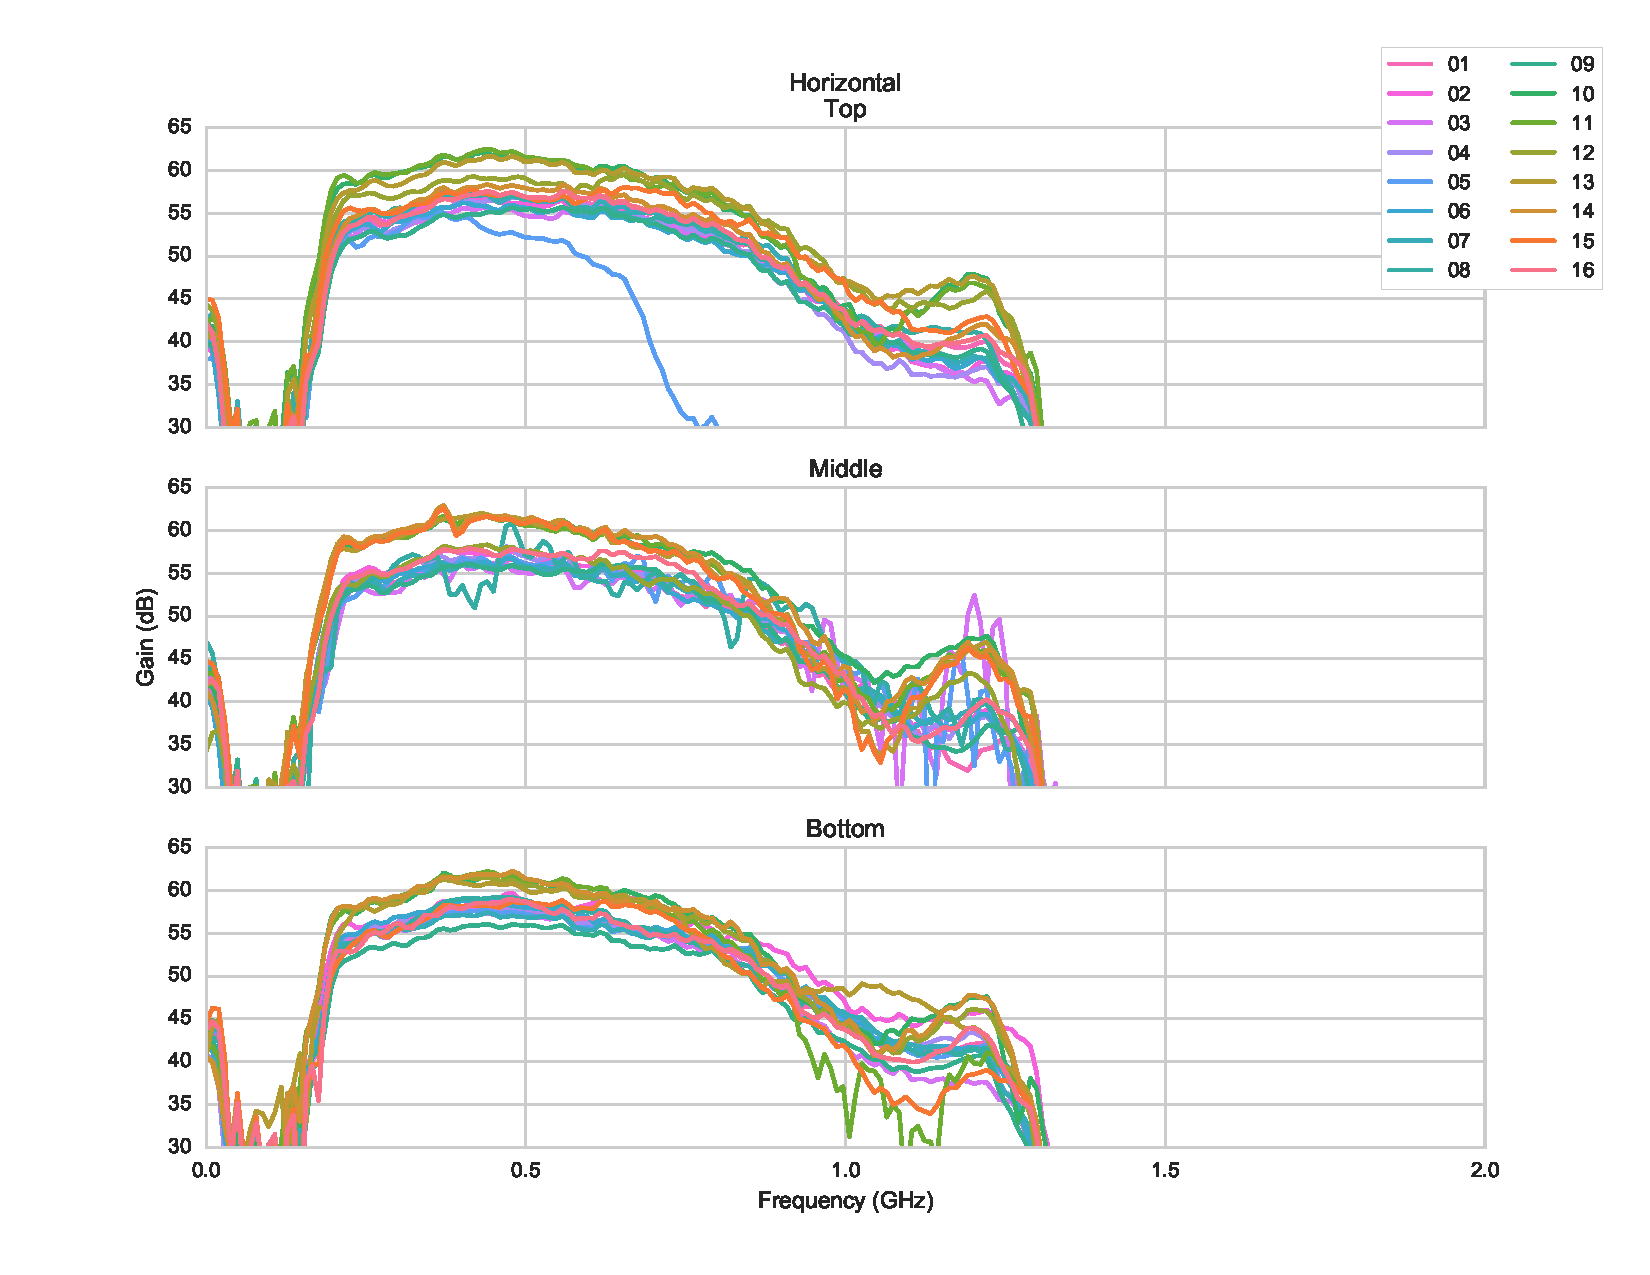
\includegraphics[width=\textwidth]{sigChain_fftH}
	\caption{Gain spectrum for the horizontally oriented polarizations of the ANITA3 signal chain.  Note 05TH, which is the ALFA antenna, and 13BH, which has been noted has an asimilar impulse response in ANITA3 and ANITA4}
\label{fig:sigChain_fftH}
\end{figure}

\begin{figure}
\centering
	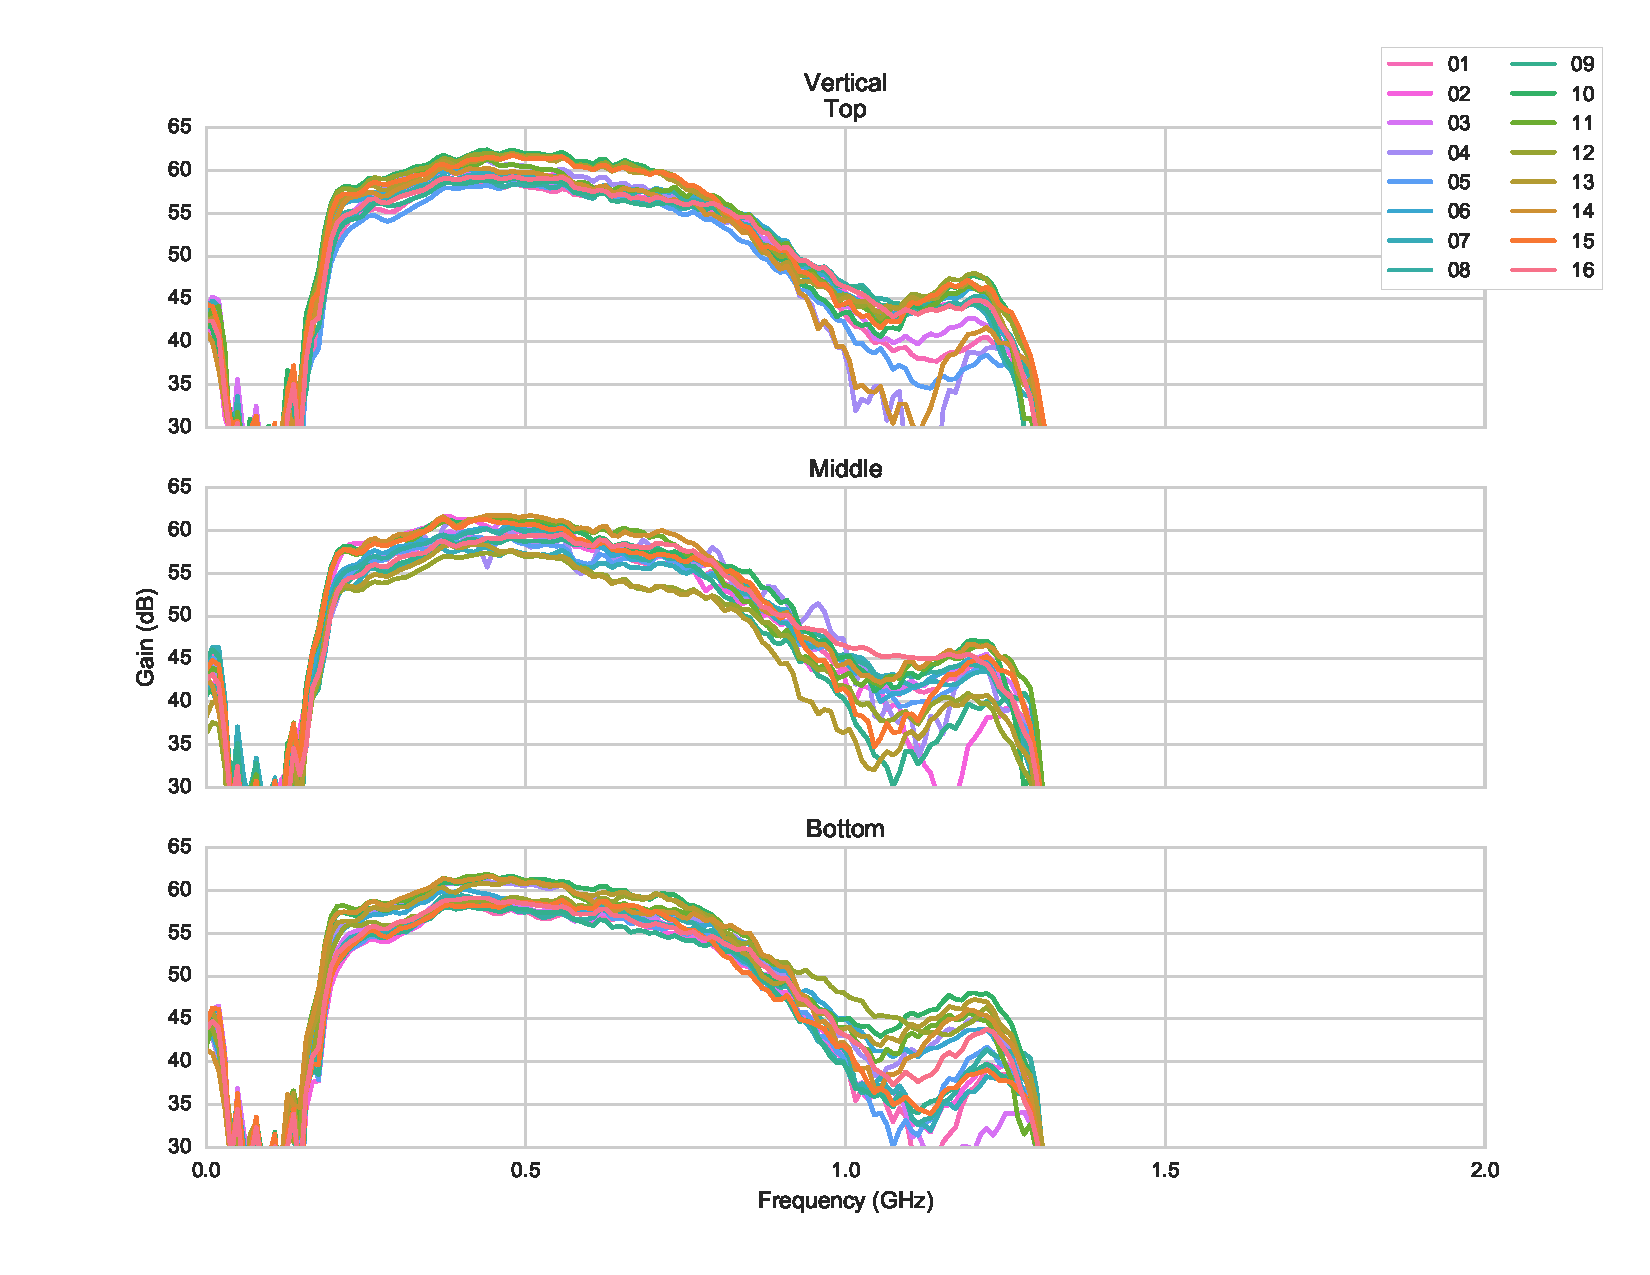
\includegraphics[width=\textwidth]{sigChain_fftV}
	\caption{Gain spectrum for the vertically oriented polarizations of the ANITA3 signal chain.}
\label{fig:sigChain_fftV}
\end{figure}
	

\section{Full Instrument Response}

	The final goal of determining the complex transfer functions for the antenna and signal chains is to relate measured ADC counts stored by the instrument into an incident electric field present on the payload.  The electric field is the true physics quantity being measured by the instrument, and a precise absolute value is desired.  Simulations of extensive air showers produced by terrestrial high energy particle interactions can generate electric field vector fields, which can be compared against our measurements only if we fully understand the full instrument response.
	
	\subsection{Convolution of antenna and signal chain}
		The convolution of the antenna normalized complex height and the signal chain complex transfer function yield the following equation:
		
\begin{equation}
V_{meas}(t) = \sqrt{\frac{50\Omega}{377\Omega}} [h_{sig}(t) \circ h_{ant}(t) \circ E_{inc}(t)] \\
\label{eqn:fullConvolution}
\end{equation}

This can be simplified by defining a global complex instrument response, $h_{inst}(t)$:

\begin{equation}
\begin{split}
h_{inst}(t) = \sqrt{\frac{Z_{c}}{Z_{o}}}h_{sig}(t) \circ h_{ant}(t) \\ 
V_{meas}(t) = h_{inst}(t) \circ E_{inc}(t)
\end{split}
\label{eqn:instTF}
\end{equation}

Solving for the instrument response yields the results shown in Figures \ref{fig:tf_H} through \ref{fig:tf_V}.  As the signal chain response is a unitless ratio of powers per frequency bin, the full instrument response takes on the units of the antenna height.  As such, I've used the naming convention normalized instrument height to describe it.

		
\begin{figure}
\centering
	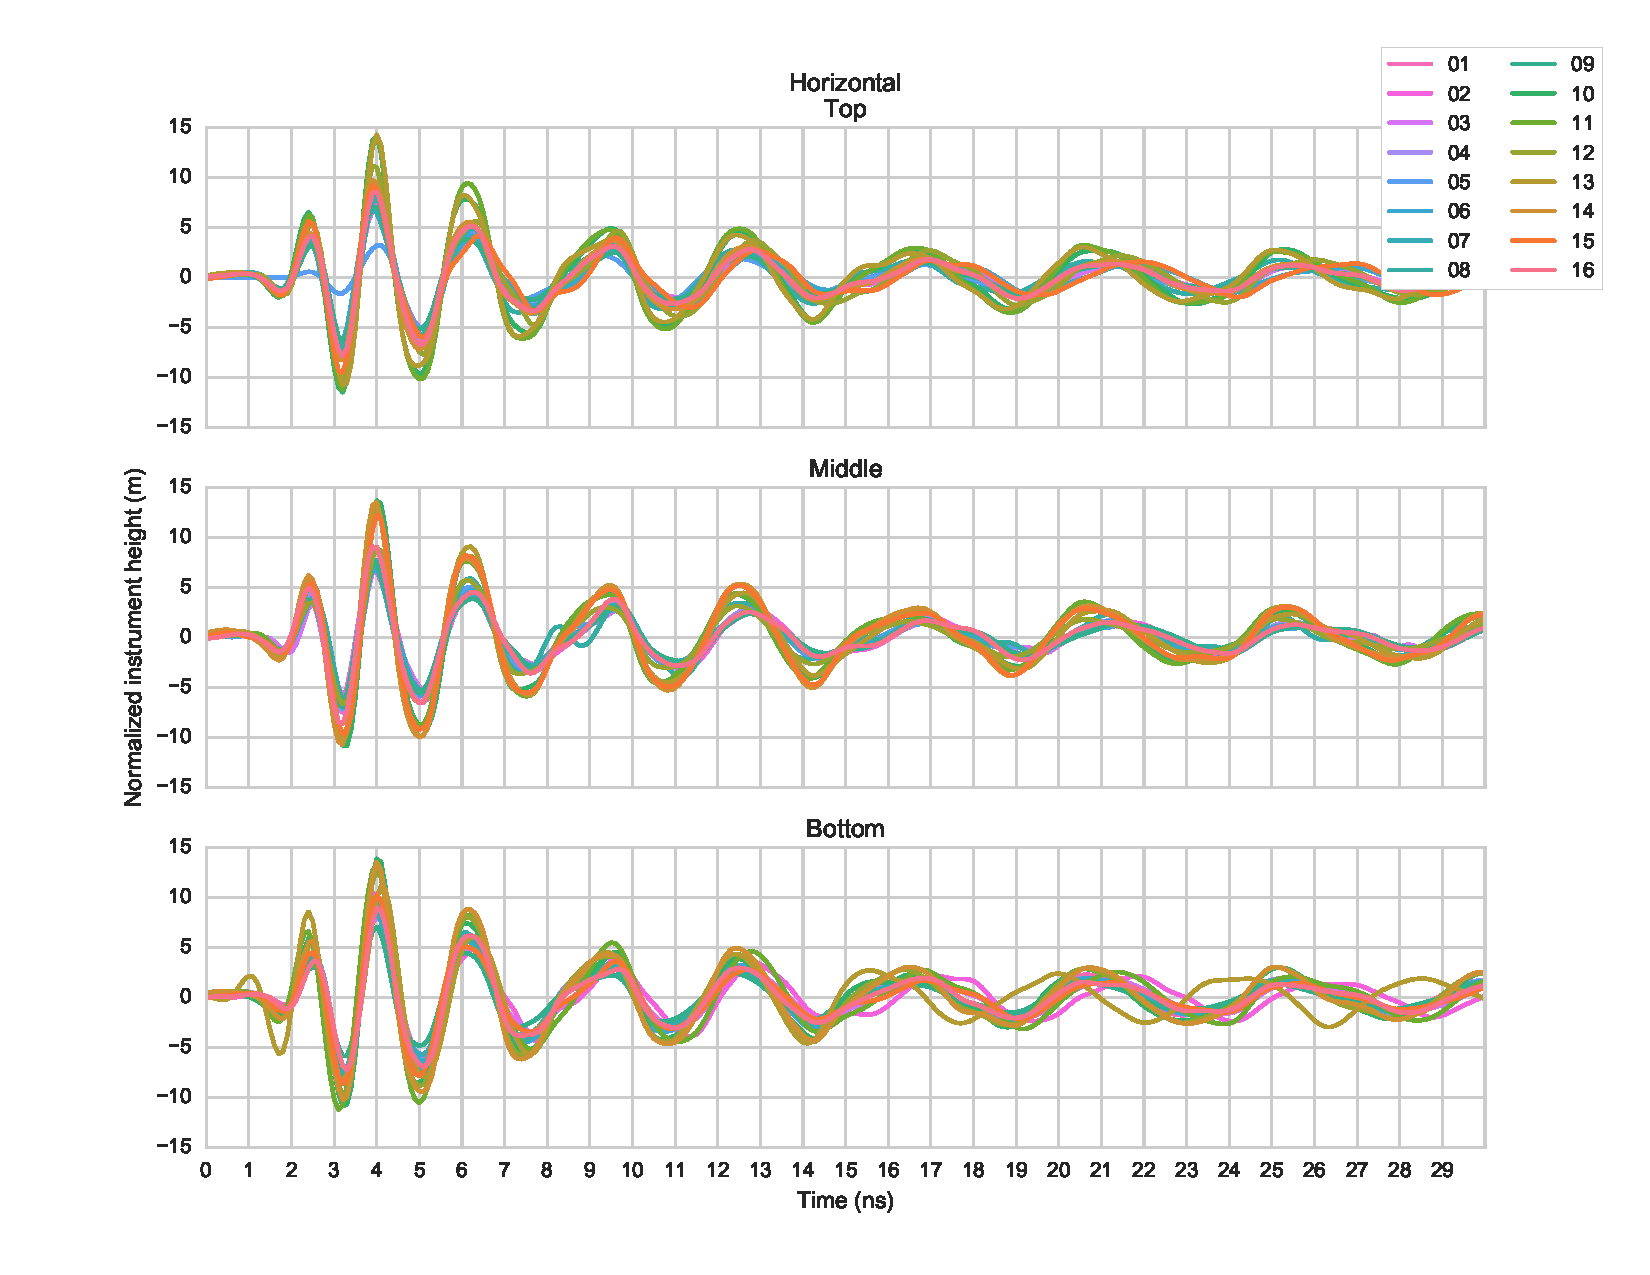
\includegraphics[width=\textwidth]{tf_timeH}
	\caption{Time domain impulse response of the horizontally oriented channels of the ANITA3 signal chain.  Note 05TH, which is the ALFA antenna, and 13BH, which has been noted has an asimilar impulse response in ANITA3 and ANITA4}
\label{fig:tf_timeH}
\end{figure}

\begin{figure}
\centering
	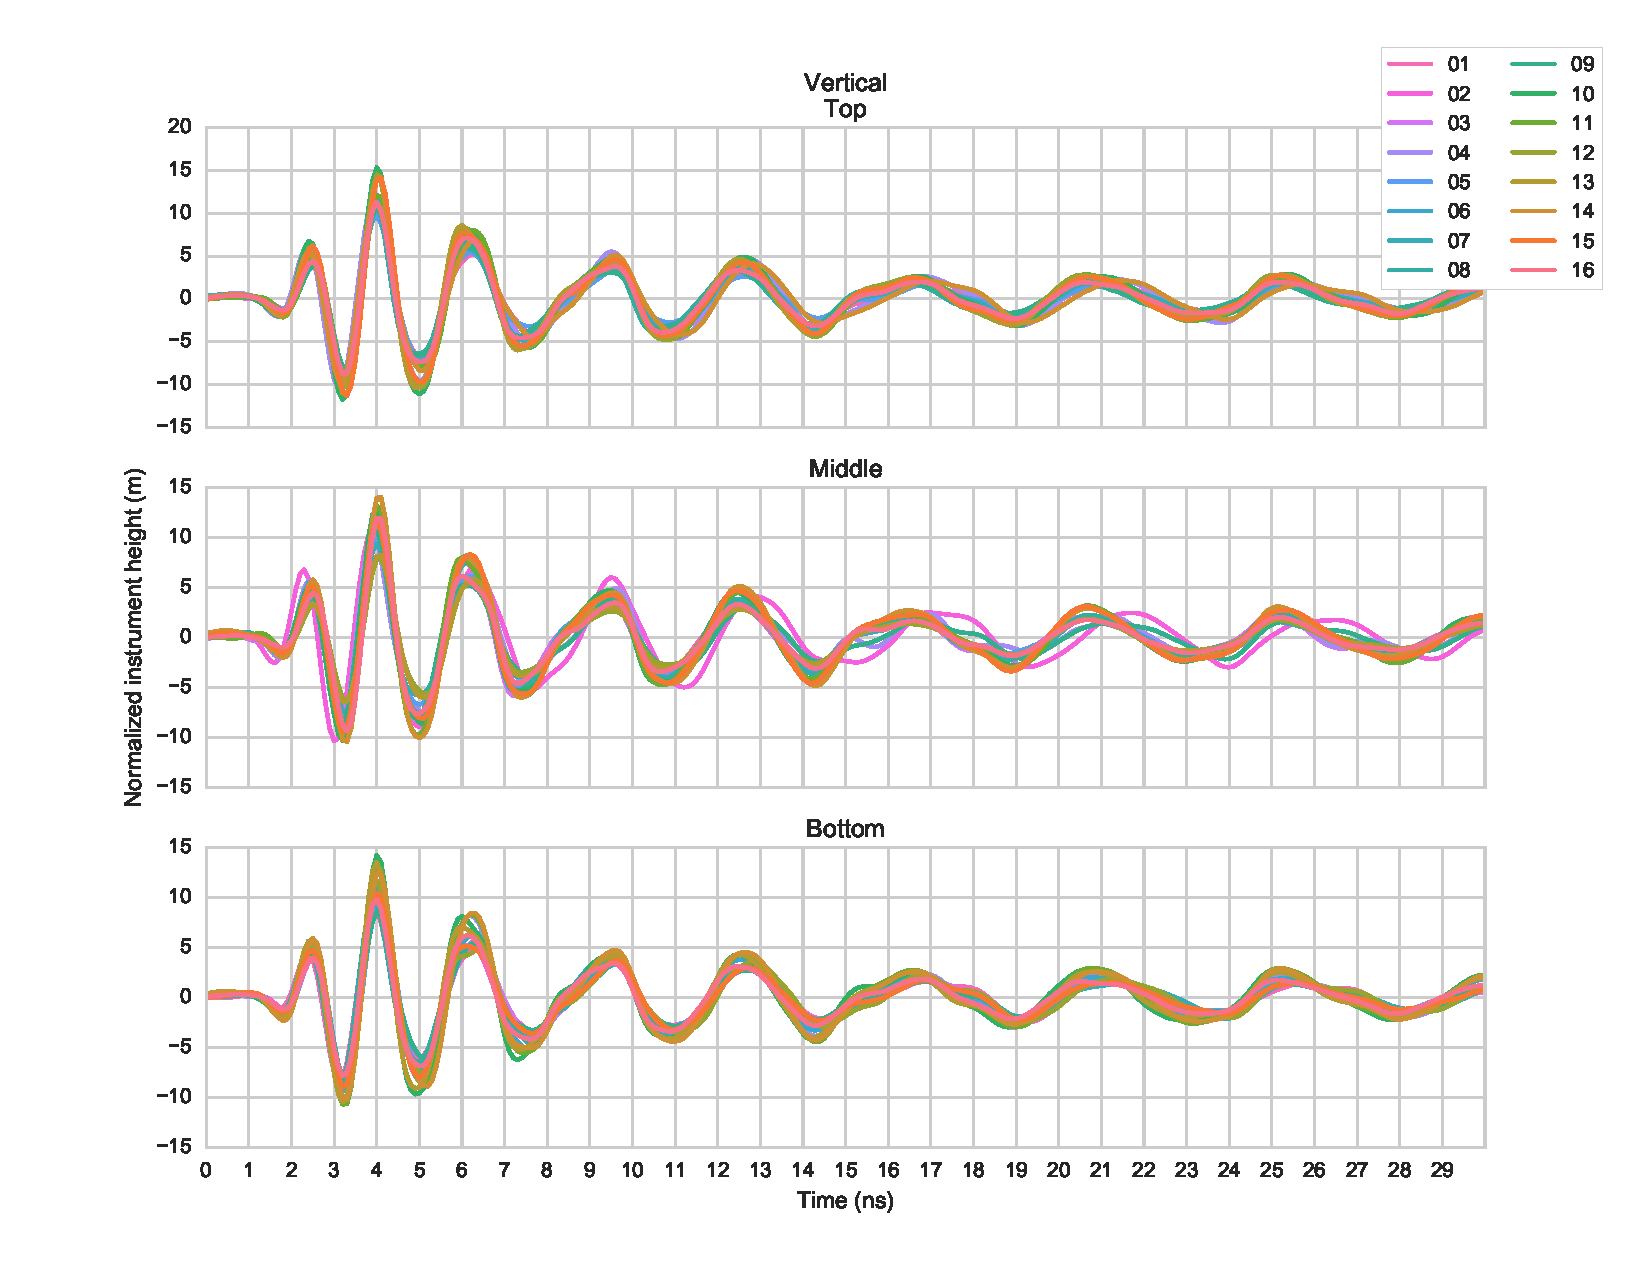
\includegraphics[width=\textwidth]{tf_timeV}
	\caption{Time domain impulse response of the vertically oriented channels of the ANITA3 signal chain.}
\label{fig:tf_timeV}
\end{figure}

\begin{figure}
\centering
	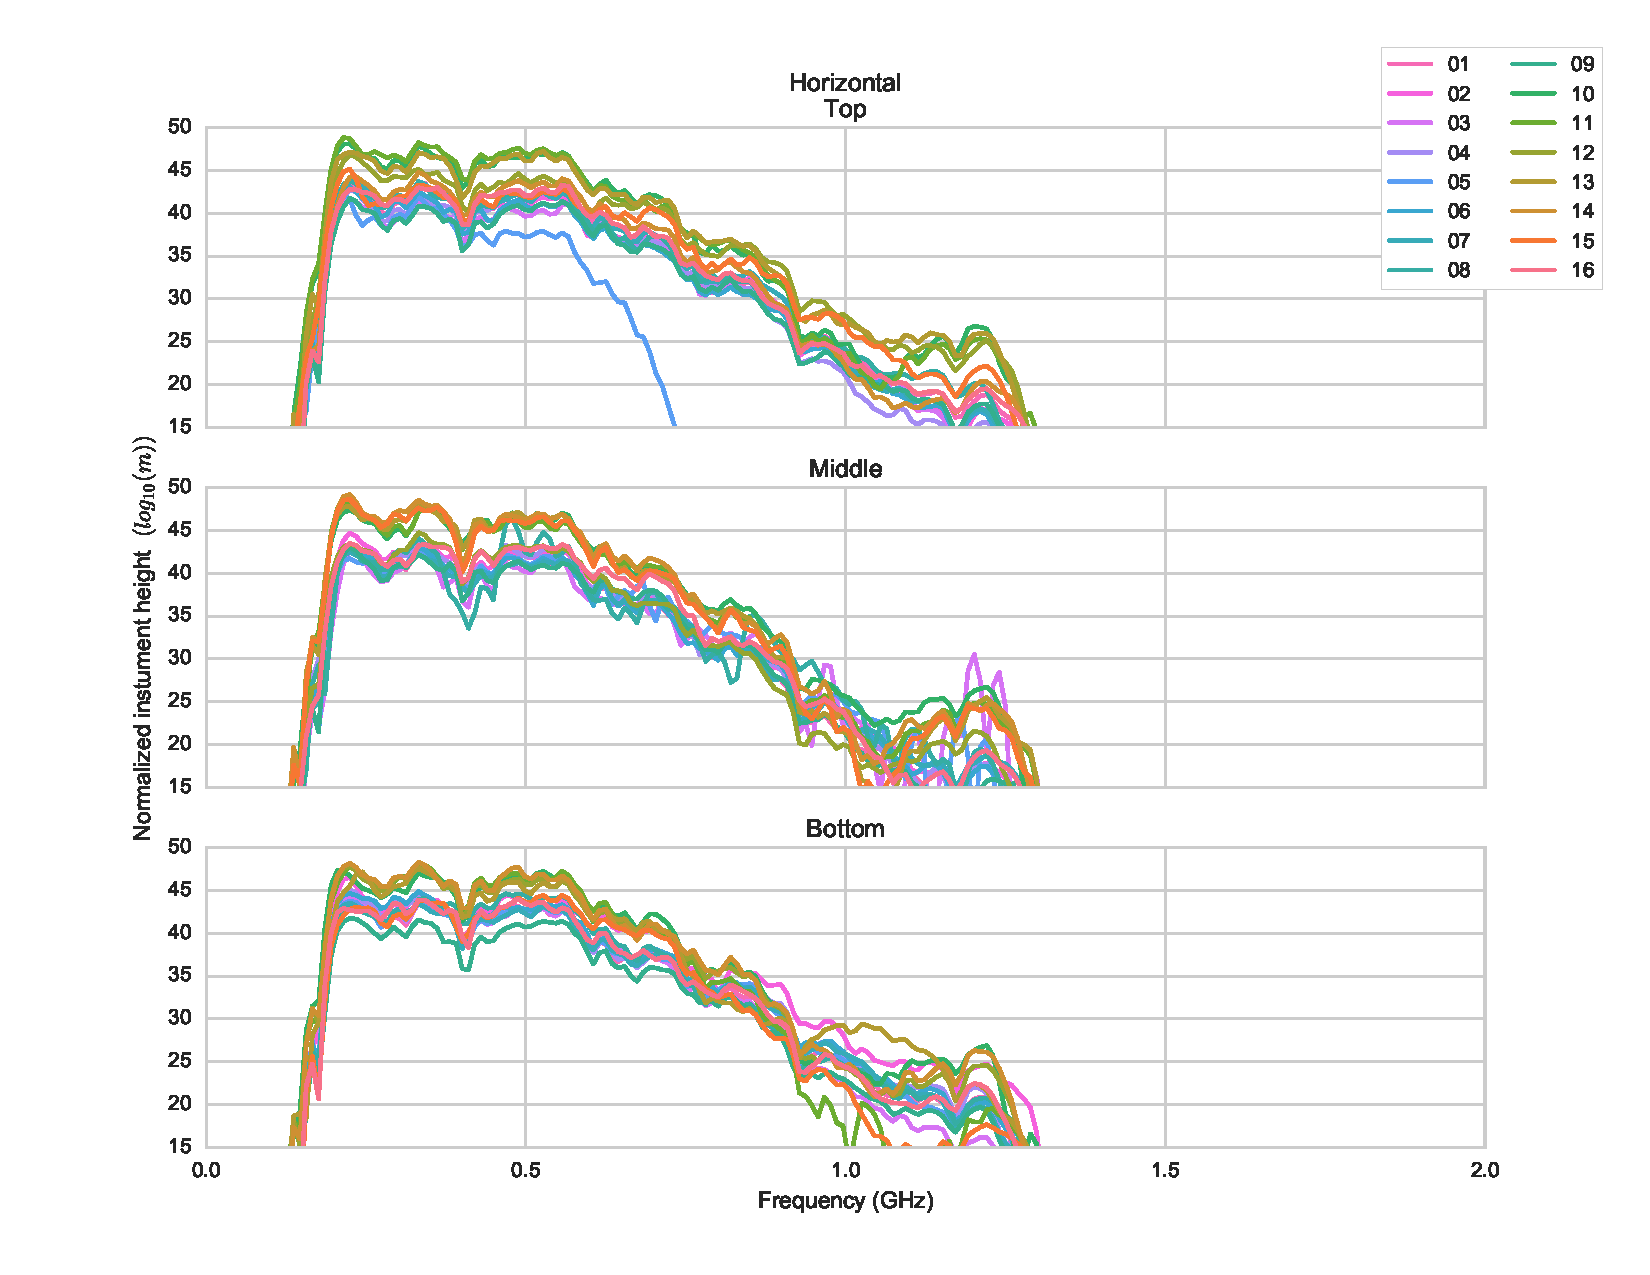
\includegraphics[width=\textwidth]{tf_fftH}
	\caption{Gain spectrum for the horizontally oriented channels of the ANITA3 signal chain.  Note 05TH, which is the ALFA antenna, and 13BH, which has been noted has an asimilar impulse response in ANITA3 and ANITA4}
\label{fig:tf_fftH}
\end{figure}

\begin{figure}
\centering
	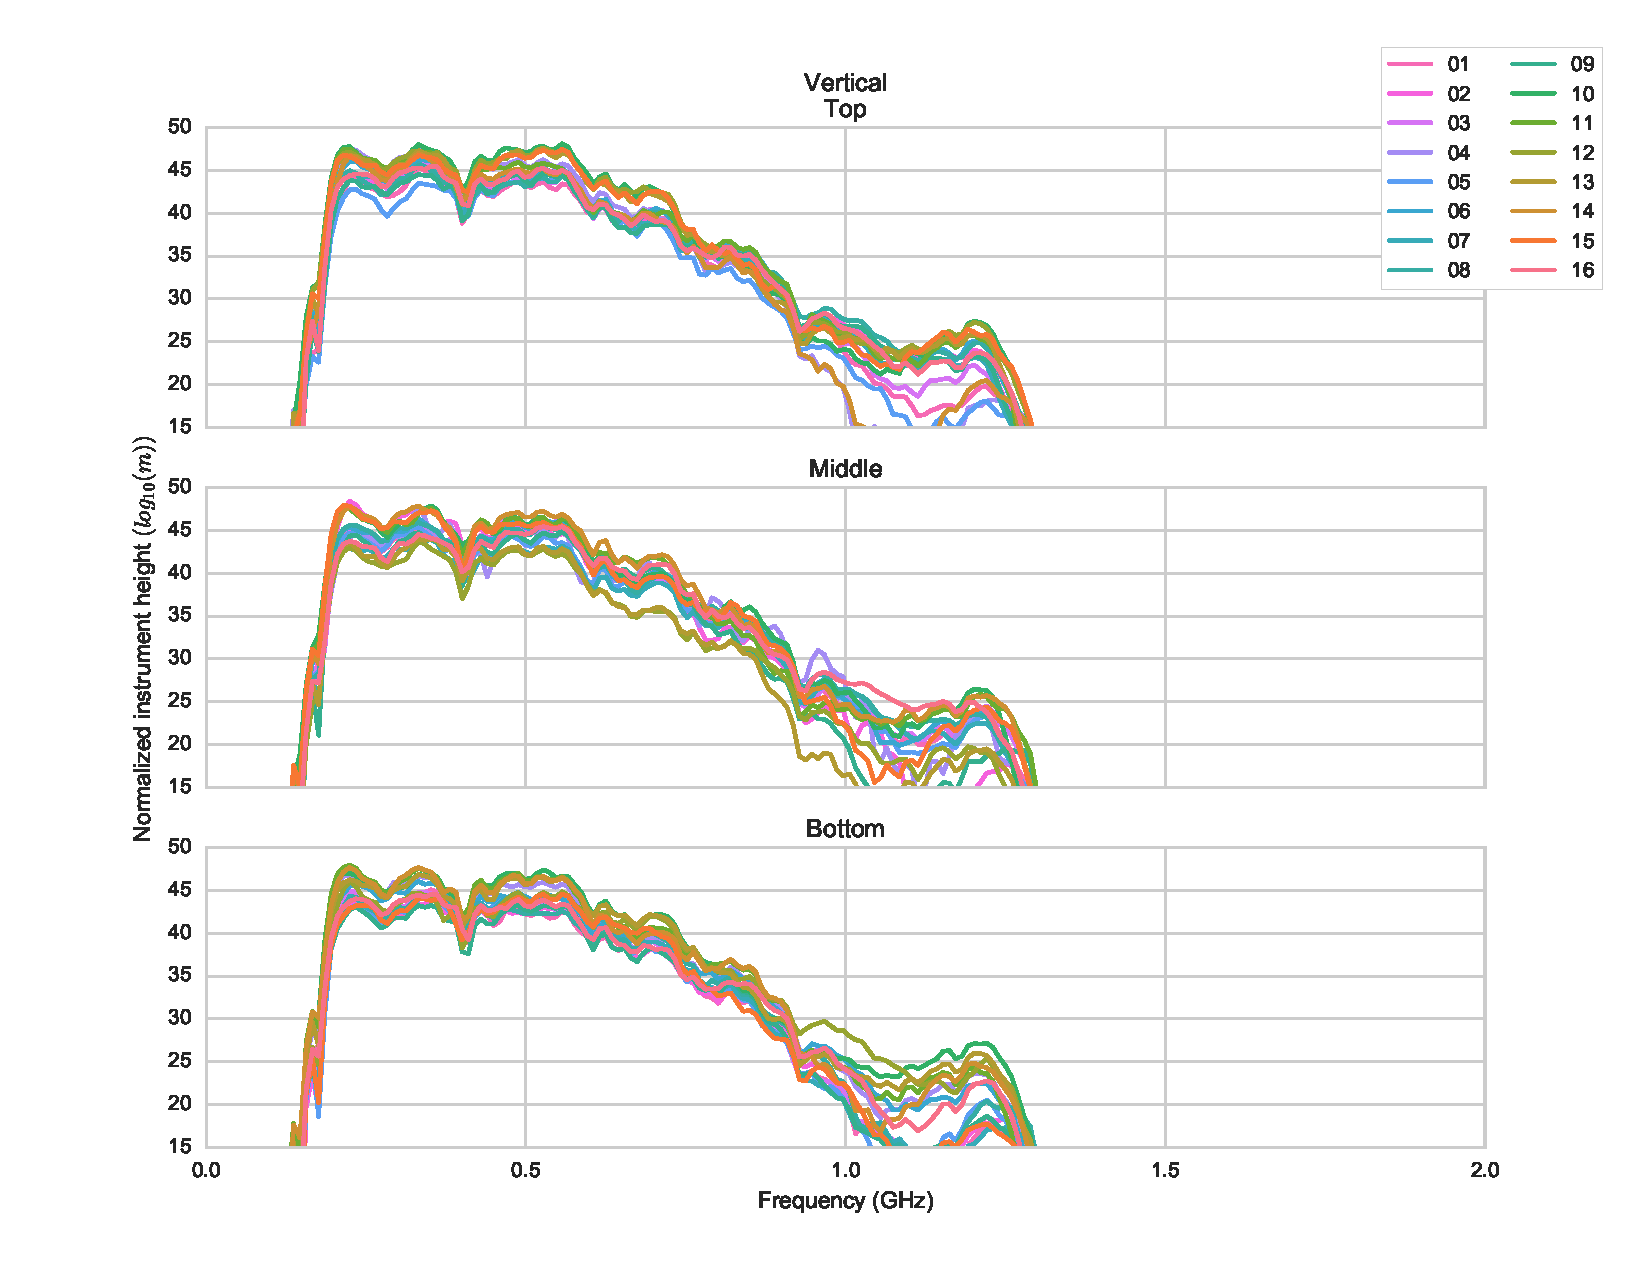
\includegraphics[width=\textwidth]{tf_fftV}
	\caption{Gain spectrum for the vertically oriented channels of the ANITA3 signal chain.}
\label{fig:tf_fftV}
\end{figure}


\section{Conclusion}
	The ANITA antenna and signal chain complex phasor responses have an overwhelming effect on the shape and magnitude of the measured air shower signal incident on the payload.  Using the processes and calibration data detailed above, that response is constrained, and signals measured by the instrument can be related back to the fundamental physics processes by which they were created.
	
